\documentclass[12pt,a4paper]{report}

\usepackage[T1]{fontenc}
\usepackage[utf8]{inputenc}
\usepackage[french]{babel}
\usepackage{lmodern,microtype}
\usepackage[a4paper,margin=2.4cm,headheight=15pt]{geometry}

\usepackage{
graphicx,float,booktabs,array,tabularx,caption,subcaption,
multirow,amsmath,siunitx,xcolor,listings,fancyhdr,
hyperref,pgfplots,enumitem
}

\newcolumntype{Y}{>{\raggedright\arraybackslash}X}

\pgfplotsset{compat=1.18}
\sisetup{locale=FR,per-mode=symbol}

\definecolor{bleu}{RGB}{20,55,95}
\definecolor{griscode}{RGB}{246,247,249}

\hypersetup{
    colorlinks=true,
    linkcolor=bleu,
    urlcolor=bleu,
    citecolor=bleu,
    pdftitle={Compte rendu TP3 - Simulation LTE et offloading de trafic WiFi/LTE},
    pdfauthor={EL JENZRI Yassine, LAMOUCHI Seif, MOUSSA Raslene, KHLIF Iheb}
}

% % --- Table des matières : profondeur chapitres + sections + sous-sections ---
\setcounter{tocdepth}{2}
\setcounter{secnumdepth}{2}

\pagestyle{fancy}
\fancyhf{}
\lhead{Protocoles des réseaux mobiles}
\rhead{TP3 -- Simulation LTE et offloading de trafic WiFi/LTE}
\cfoot{\thepage}

\setlength{\parskip}{5pt}
\setlength{\parindent}{0pt}

\lstset{
    basicstyle=\ttfamily\small,
    backgroundcolor=\color{griscode},
    frame=single,
    breaklines=true,
    columns=fullflexible,
    showstringspaces=false
}

\newcommand{\capture}[3]{
\begin{figure}[H]
\centering
\IfFileExists{#1}{
    \includegraphics[width=.96\textwidth,height=.58\textheight,keepaspectratio]{#1}
}{
    \fbox{
        \parbox{.88\textwidth}{
            \centering
            \vspace{1cm}
            \textbf{Capture à ajouter :}
            \texttt{#1}
            \vspace{1cm}
        }
    }
}
\caption{#2}
\label{#3}
\end{figure}
}
\newcommand{\todo}[1]{\textit{[À compléter après réalisation et mesure : #1]}}

\begin{document}

% ==================================================
% PAGE DE GARDE
% ==================================================

\pagenumbering{gobble}

\begin{titlepage}
\centering

\noindent
\begin{minipage}[c]{0.46\textwidth}
\centering
\IfFileExists{universite-de-carthage.png}{
    
\includegraphics[height=4cm,keepaspectratio]{universite-de-carthage.png}
}{
    \fbox{
        \parbox[c][2.2cm][c]{0.88\linewidth}{
            \centering Logo\\Université de Carthage
        }
    }
}
\end{minipage}
\hfill
\begin{minipage}[c]{0.46\textwidth}
\centering
\IfFileExists{logo-insat.jpg}{
    
\includegraphics[height=3.5cm,keepaspectratio]{logo-insat.jpg}
}{
    \fbox{
        \parbox[c][2.2cm][c]{0.88\linewidth}{
            \centering Logo\\INSAT
        }
    }
}
\end{minipage}

\par\vspace{.35cm}

{\large Ministère de l'Enseignement Supérieur et de la Recherche Scientifique\par}
\vspace{.35cm}

{\large Université de Carthage\par}
\vspace{.2cm}

{\large Institut National des Sciences Appliquées et de Technologie (INSAT)\par}

\vspace{.7cm}
{\color{bleu}\rule{\textwidth}{1.3pt}}
\vspace{.3cm}

{\Huge\bfseries COMPTE RENDU DU TP3\par}
\vspace{.2cm}

{\LARGE Protocoles des réseaux mobiles\par}
\vspace{.3cm}

{\color{bleu}\rule{\textwidth}{1.3pt}}
\vspace{.65cm}

{\huge\bfseries Simulation LTE et offloading de trafic WiFi/LTE\par}

\vspace{.75cm}
{\Large\textbf{Réalisé par}\par}
\vspace{.25cm}

{\Large EL JENZRI Yassine\par}
\vspace{.08cm}
{\Large LAMOUCHI Seif\par}
\vspace{.08cm}
{\Large MOUSSA Raslene\par}
\vspace{.08cm}
{\Large KHLIF Iheb\par}

\vfill

\begin{tabular}{rl}
\textbf{Matière :} & Protocoles des réseaux mobiles\\
\textbf{Niveau :} & Cycle ingénieur -- RT4\\
\textbf{Responsable du cours et TP :} & Dr Mériem Afif\\
\textbf{Année universitaire :} & 2026--2027
\end{tabular}

\vspace{.45cm}

\end{titlepage}

% ==================================================
% TABLE DES MATIERES
% ==================================================

\pagenumbering{roman}
\setcounter{page}{1}
\tableofcontents
\clearpage
\pagenumbering{arabic}

% ==================================================
% PARTIE A -- Architecture et simulation LTE/EPC
% Auteur : KHLIF Iheb
% Les figures sont dans img/A/ (chemins relatifs au fichier principal).
% ==================================================

\chapter{Partie A --- Architecture et simulation LTE/EPC}

Cette partie présente l'architecture LTE/EPC telle qu'elle est modélisée dans
NS-3 (version 3.48), la simulation d'une communication de bout en bout, puis
l'influence de la distance, de la mobilité et du handover sur le débit et sur la
puissance reçue (RSRP). Les six questions du TP sont traitées dans l'ordre de
l'énoncé.

\section*{Paramètres communs aux simulations}

Sauf mention contraire, toutes les simulations de cette partie reposent sur le
même squelette, dérivé de l'exemple \texttt{lena-simple-epc.cc} (fichiers
\texttt{tp3\_q1.cc}, \texttt{tp3\_q5.cc}, \texttt{tp3\_q5\_parallel.cc} et
\texttt{tp3\_q6.cc}).

\begin{table}[H]
\centering
\caption{Paramètres communs des simulations de la partie A.}
\label{tab:A-params}
\small
\begin{tabularx}{\textwidth}{@{}lY@{}}
\toprule
\textbf{Élément} & \textbf{Valeur} \\
\midrule
Topologie & 1 eNodeB en $(0,0,0)$, 1 UE, 1 remote host relié au PGW
(liaison point-à-point de \SI{100}{Gb/s}, délai \SI{10}{ms}, MTU 1500) \\
Trafic & Deux flux UDP simultanés générés par \texttt{UdpClient} avec un
paquet toutes les \SI{1}{ms} (taille par défaut de \SI{1024}{o}) :
descendant (remote host $\rightarrow$ UE, port 1100) et montant
(UE $\rightarrow$ remote host, port 2001), démarrés à \SI{0.5}{s} \\
Charge offerte & $(1024+8+20+4)\times 8 / \SI{1}{ms} = \SI{8.448}{Mb/s}$
par sens au niveau RLC (1024 o de données, 8 o UDP, 20 o IP, environ 4 o
d'en-têtes PDCP/RLC) ; \SI{8.416}{Mb/s} au niveau IP \\
Couche radio & Paramètres par défaut du module LTE : modèle de propagation
de Friis, porteuse à \SI{2.12}{GHz}, 25 blocs de ressources (\SI{5}{MHz}),
puissance d'émission de \SI{30}{dBm} (eNodeB) et \SI{10}{dBm} (UE) \\
Traces & \texttt{lteHelper->EnableTraces()} (fichiers \texttt{DlRlcStats} et
\texttt{UlRlcStats}), \texttt{lteHelper->EnablePhyTraces()} (fichier
\texttt{DlRsrpSinrStats}) et FlowMonitor \\
\bottomrule
\end{tabularx}
\end{table}

Le choix d'une charge de \SI{8.4}{Mb/s} par sens est important pour
l'interprétation des résultats : c'est une charge \emph{fixe} (débit constant),
inférieure à la capacité maximale de la cellule. Le débit mesuré ne peut donc
jamais dépasser \SI{8.4}{Mb/s} et il ne diminue que lorsque la capacité du lien
radio devient inférieure à cette charge.

% ==================================================
\section{Question 1 --- Simulation LTE/EPC et connectivité de bout en bout}
% ==================================================

\subsection{Principe du scénario}

Le scénario construit suit la chaîne
\emph{Remote host} $\leftrightarrow$ \emph{PGW/SGW} $\leftrightarrow$
\emph{eNodeB} $\leftrightarrow$ \emph{UE}. Le cœur de réseau est instancié par
\texttt{PointToPointEpcHelper}, la partie radio par \texttt{LteHelper}. Les
étapes principales sont les suivantes :

\begin{enumerate}[nosep]
\item création des deux helpers et de la liaison entre l'EPC et le
\texttt{LteHelper} (\texttt{SetEpcHelper}) ;
\item création du remote host, installation de la pile Internet et connexion au
PGW par une liaison point-à-point ;
\item création d'un eNodeB et d'un UE, placés par un modèle de mobilité à
position constante ;
\item installation des équipements LTE, attribution d'une adresse IP à l'UE par
le PGW (\texttt{AssignUeIpv4Address}) et attachement de l'UE à l'eNodeB ;
\item configuration du routage statique : route vers le réseau \texttt{7.0.0.0/8}
(réseau des UE) sur le remote host, et passerelle par défaut de l'UE vers le
PGW ;
\item installation des applications (flux UDP, ping) et activation des traces.
\end{enumerate}

\begin{lstlisting}[language=C++]
Ptr<LteHelper> lteHelper = CreateObject<LteHelper>();
Ptr<PointToPointEpcHelper> epcHelper = CreateObject<PointToPointEpcHelper>();
lteHelper->SetEpcHelper(epcHelper);

// Routage : le remote host joint le reseau des UE via le PGW ;
// l'UE utilise le PGW comme passerelle par defaut.
remoteHostStaticRouting->AddNetworkRouteTo(Ipv4Address("7.0.0.0"),
                                           Ipv4Mask("255.0.0.0"), 1);
ueStaticRouting->SetDefaultRoute(epcHelper->GetUeDefaultGatewayAddress(), 1);

lteHelper->Attach(ueLteDevs.Get(0), enbLteDevs.Get(0));

PingHelper ping(ueIpIface.GetAddress(0));   // remote host -> UE
lteHelper->EnableTraces();
lteHelper->EnablePhyTraces();
\end{lstlisting}

\subsection{Vérification par ping}

Un ping est lancé depuis le remote host vers l'UE (adresse \texttt{7.0.0.2},
attribuée par le PGW dans le réseau \texttt{7.0.0.0/8}). Le résultat est
présenté en figure~\ref{fig:A-ping}.

\capture{img/A/q1-ping.png}{Ping du remote host vers l'UE (adresse
\texttt{7.0.0.2}) : connectivité de bout en bout vérifiée.}{fig:A-ping}

La connectivité de bout en bout est établie : les quatre requêtes reçoivent une
réponse, sans perte. Deux observations méritent d'être commentées :

\begin{itemize}[nosep]
\item \textbf{TTL = 63.} Le TTL initial (64) est décrémenté d'une unité : le
paquet a traversé un seul routeur IP, le PGW. Le tunnel GTP-U entre le PGW et
l'eNodeB est transparent pour la couche IP de bout en bout, ce qui est
précisément le rôle de l'encapsulation GTP-U.
\item \textbf{RTT d'environ \SI{29}{ms} à \SI{32}{ms}.} La liaison PGW--remote
host introduit à elle seule $2\times\SI{10}{ms}=\SI{20}{ms}$. Les \SI{9}{ms}
à \SI{12}{ms} restants correspondent à la traversée de l'interface radio (en
LTE, la transmission est organisée en sous-trames de \SI{1}{ms} ; l'ordonnancement
descendant et surtout la procédure d'allocation montante -- demande
d'ordonnancement puis attribution de ressources -- ajoutent quelques
millisecondes) ainsi qu'au traitement dans les couches PDCP/RLC/MAC. L'alternance
entre \SI{28.9}{ms} et \SI{31.9}{ms} (écart de \SI{3}{ms}) provient de
l'alignement des paquets sur la cadence des sous-trames et des opportunités
d'émission montante.
\end{itemize}

% ==================================================
\section{Question 2 --- Rôle des entités de l'architecture EPC simulée}
% ==================================================

La figure~\ref{fig:A-archi} résume l'architecture simulée. NS-3 sépare le réseau
d'accès radio (E-UTRAN, constitué des eNodeB) du cœur de réseau (EPC).

\begin{figure}[H]
\centering
\begin{tikzpicture}[
  ent/.style={draw=bleu, fill=bleu!8, rounded corners=3pt, minimum width=2.0cm,
              minimum height=1.0cm, align=center, font=\small\bfseries},
  autre/.style={ent, dashed, fill=white, font=\small},
  lien/.style={thick, bleu},
  lbl/.style={font=\scriptsize, align=center, text=black}]
  \node[ent] (ue)  at (0,0)    {UE};
  \node[ent] (enb) at (4.6,0)  {eNodeB};
  \node[ent] (gw)  at (9.2,0)  {SGW/PGW};
  \node[ent] (rh)  at (13.6,0) {Remote\\host};
  \node[ent]   (mme)  at (6.9,2.8) {MME};
  \node[autre] (enb2) at (2.0,2.8) {autre\\eNodeB};

  \draw[lien] (ue) -- (enb) node[midway, above=1pt, lbl] {Uu};
  \node[lbl, below=2pt] at (2.3,0) {PDCP/RLC/\\MAC/PHY};
  \draw[lien] (enb) -- (gw) node[midway, above=1pt, lbl] {S1-U};
  \node[lbl, below=2pt] at (6.9,0) {GTP-U/\\UDP/IP};
  \draw[lien] (gw) -- (rh) node[midway, above=1pt, lbl] {SGi (IP)};
  \node[lbl, below=2pt] at (11.4,0) {100~Gb/s\\10~ms};
  \draw[lien, dashed] (enb2) -- (enb) node[midway, above, sloped, lbl] {X2};
  \draw[lien] (enb) -- (mme) node[midway, above, sloped, lbl] {S1-MME};
  \draw[lien] (mme) -- (gw) node[midway, above, sloped, lbl] {S11};

  \draw[<->, thick, orange!80!black] (0,-1.7) -- (9.2,-1.7)
    node[midway, below, lbl] {porteuse EPS = porteuse radio (Uu) + tunnel GTP-U (S1-U)};
  \draw[<->, thick, green!50!black] (0,-2.7) -- (13.6,-2.7)
    node[midway, below, lbl] {connexion IP de bout en bout (UE \texttt{7.0.0.2} $\leftrightarrow$ remote host \texttt{1.0.0.2})};
\end{tikzpicture}
\caption{Architecture LTE/EPC simulée sous NS-3 : entités, interfaces et
piles protocolaires du plan usager.}
\label{fig:A-archi}
\end{figure}

\begin{description}[style=nextline, leftmargin=1.2em, itemsep=4pt]
\item[eNodeB (station de base).] C'est l'unique entité de l'E-UTRAN. Elle porte
la pile radio PDCP/RLC/MAC/PHY avec les UE de sa cellule (interface Uu) et gère
les ressources radio : ordonnancement (scheduler MAC), adaptation du débit
(choix du MCS selon la qualité du canal), contrôle des mesures et décision de
handover (RRC). Côté réseau, l'eNodeB relie chaque porteuse radio à un tunnel
GTP-U vers la passerelle : il est le point de jonction entre le monde radio et
le monde IP.

\item[SGW (Serving Gateway).] Passerelle de données du côté accès. Elle termine
les tunnels GTP-U venant des eNodeB et sert de point d'ancrage pour la mobilité
entre eNodeB : lors d'un handover (Q6), c'est la SGW qui redirige le tunnel
descendant vers le nouvel eNodeB sans que l'adresse IP de l'UE ne change.

\item[PGW (PDN Gateway).] Passerelle vers le réseau extérieur (ici, le remote
host). Elle attribue l'adresse IP de l'UE (réseau \texttt{7.0.0.0/8}),
encapsule dans un tunnel GTP-U les paquets descendants destinés à l'UE
(sélection de la porteuse EPS adaptée) et décapsule les paquets montants avant
de les router vers Internet. C'est elle qui apparaît comme routeur dans le
ping (TTL = 63). Dans NS-3, SGW et PGW sont regroupées dans un seul n\oe ud
(\texttt{GetPgwNode()}).

\item[MME (Mobility Management Entity).] Entité de contrôle : attachement de
l'UE, établissement des porteuses EPS et gestion de la mobilité. Dans NS-3 elle
est fortement simplifiée : la signalisation S1-MME est modélisée par des
échanges directs entre entités et non par une liaison simulée.

\item[Interface S1.] Elle relie les eNodeB à l'EPC. Sa partie plan usager,
S1-U, transporte les paquets IP de l'UE dans des tunnels GTP-U (GTP-U sur UDP
sur IP) entre l'eNodeB et la SGW/PGW ; sa partie plan de contrôle, S1-MME,
véhicule la signalisation vers la MME. Dans NS-3, S1-U est simulée par une
liaison point-à-point dédiée par eNodeB. L'interface X2, entre eNodeB voisins,
sera utilisée à la question~6 pour le handover.
\end{description}

\paragraph{Parcours d'un paquet descendant.} Le remote host émet un paquet vers
\texttt{7.0.0.2} ; le PGW le reçoit comme routeur, l'encapsule dans le tunnel
GTP-U de la porteuse EPS de l'UE ; il traverse S1-U jusqu'à l'eNodeB, qui le
décapsule puis le transmet à l'UE par les couches PDCP, RLC, MAC et PHY.
Le chemin inverse est suivi par les paquets montants. La couche IP de l'UE et
celle du remote host voient une simple connexion de bout en bout, comme le
montre la figure de la pile protocolaire de l'énoncé.

% ==================================================
\section{Question 3 --- Débit descendant et montant en fonction du temps}
% ==================================================

Les fichiers \texttt{DlRlcStats.txt} et \texttt{UlRlcStats.txt} fournissent,
par intervalle de \SI{0.25}{s}, le nombre d'octets reçus au niveau RLC. Le débit
est calculé pour chaque intervalle $[t_{d}, t_{f}]$ par
\[
  D = \frac{8 \times \text{RxBytes}}{t_{f}-t_{d}}
\]
et rapporté au milieu de l'intervalle (script \texttt{tp3\_q3.py}). La
simulation dure \SI{5}{s} avec l'UE fixe à \SI{60}{m} de l'eNodeB. Le résultat
est donné en figure~\ref{fig:A-q3}.

\capture{img/A/q3-debit-temps.png}{Débit LTE descendant (haut) et montant
(bas) en fonction du temps, d'après \texttt{DlRlcStats} et
\texttt{UlRlcStats}.}{fig:A-q3}

\paragraph{Interprétation.}
\begin{itemize}[nosep]
\item \textbf{Régime permanent.} Le débit descendant se stabilise à
\SI{8.45}{Mb/s}, valeur qui correspond exactement à la charge offerte au niveau
RLC (\SI{8.448}{Mb/s}, tableau~\ref{tab:A-params}). À \SI{60}{m} de l'eNodeB le
canal est excellent : la cellule écoule tout le trafic offert, sans perte. Le
plateau n'est donc pas la capacité de la cellule, mais la charge imposée par la
source UDP.
\item \textbf{Phase transitoire.} Le premier échantillon (environ
\SI{8.0}{Mb/s}) est plus faible : la source démarre à \SI{0.5}{s} et ses
premiers paquets n'arrivent à l'UE qu'après un délai d'une douzaine de
millisecondes (\SI{10}{ms} de liaison Internet auxquelles s'ajoute le délai
radio), ce qui retire environ 5\,\% de volume à l'intervalle
$[0.5\,;\,0.75]$~s.
\item \textbf{Variations du débit montant.} Le débit montant oscille entre
environ \SI{8.2}{Mb/s} et \SI{8.65}{Mb/s} autour de la même valeur moyenne
(\SI{8.45}{Mb/s}). Ces variations d'environ $\pm 3\,\%$ ne traduisent pas une
instabilité du lien : en montant, l'UE ne peut émettre que dans les ressources
que l'eNodeB lui attribue sous forme de blocs de transport discrets (demande
d'ordonnancement, rapport d'état du tampon, puis attribution). Les paquets
sont donc écoulés par rafales, et le nombre d'octets qui tombe dans chaque
fenêtre de \SI{0.25}{s} varie légèrement, alors que la moyenne reste égale au
débit offert. En descendant, l'ordonnanceur de l'eNodeB dispose directement du
tampon et lisse davantage la livraison.
\end{itemize}

% ==================================================
\section{Question 4 --- Influence de la distance UE--eNodeB}
% ==================================================

\subsection{Méthodologie}

L'UE est placé à position constante sur l'axe $x$ à une distance $d$ de
l'eNodeB. Le script \texttt{tp3\_q4.py} lance la simulation pour
$d \in \{100;\,300;\,500;\,1000;\,1500;\,2000;\,3000;\,4000;\,5000;\,6000;\,7000;\,8000;\,9000;\,10000\}$~m
(paramètre \texttt{--distance} de \texttt{tp3\_q1}) puis, pour chaque run :
\begin{itemize}[nosep]
\item le débit moyen DL et UL est calculé à partir de \texttt{DlRlcStats} et
\texttt{UlRlcStats} (octets reçus divisés par la durée) ;
\item le RSRP est lu dans \texttt{DlRsrpSinrStats} (colonne en watts) ; les
échantillons sont moyennés en puissance linéaire, puis convertis en dBm.
\end{itemize}

\subsection{Résultats}

\capture{img/A/q4-debit-distance.png}{Débit moyen descendant et montant en
fonction de la distance UE--eNodeB.}{fig:A-q4-debit}

\capture{img/A/q4-rsrp-distance.png}{RSRP moyen en fonction de la distance
UE--eNodeB.}{fig:A-q4-rsrp}

\begin{table}[H]
\centering
\caption{Valeurs caractéristiques relevées sur les figures~\ref{fig:A-q4-debit}
et~\ref{fig:A-q4-rsrp} (valeurs approchées) et RSRP théorique du modèle de
Friis.}
\label{tab:A-q4}
\small
\begin{tabular}{rcccc}
\toprule
Distance (m) & RSRP simulé (dBm) & RSRP Friis (dBm) & Débit DL (Mb/s) & Débit UL (Mb/s) \\
\midrule
100    & $-73{,}8$  & $-73{,}7$  & 8,42 & 8,44 \\
1000   & $-93{,}8$  & $-93{,}7$  & 8,42 & 8,44 \\
4000   & $-105{,}8$ & $-105{,}8$ & 8,42 & 8,44 \\
5000   & $-107{,}7$ & $-107{,}7$ & 8,42 & 6,43 \\
6000   & $-109{,}3$ & $-109{,}3$ & 8,42 & 4,95 \\
7000   & $-110{,}6$ & $-110{,}6$ & 7,7  & 4,95 \\
8000   & $-111{,}8$ & $-111{,}8$ & 7,2  & 4,38 \\
9000   & $-112{,}8$ & $-112{,}8$ & 7,2  & 3,49 \\
10000  & $-113{,}7$ & $-113{,}7$ & 6,18 & 3,49 \\
\bottomrule
\end{tabular}
\end{table}

\subsection{Interprétation}

\paragraph{Le RSRP suit la loi de Friis.} Le RSRP décroît de
\SI{-73.8}{dBm} à \SI{100}{m} jusqu'à \SI{-113.7}{dBm} à \SI{10}{km}, soit
\SI{20}{dB} par décade de distance : c'est la signature d'une propagation en
espace libre (exposant d'affaiblissement $n=2$). La puissance d'émission de
\SI{30}{dBm} est répartie sur $25\times12=300$ éléments de ressource, d'où une
puissance de référence par élément de $30-10\log_{10}300 \approx \SI{5.2}{dBm}$,
et
\[
  \mathrm{RSRP}(d) \approx 5{,}2 - 20\log_{10}\!\left(\frac{4\pi d f}{c}\right)
  \quad\text{avec } f=\SI{2.12}{GHz},
\]
soit $-73{,}7$~dBm à \SI{100}{m} et $-113{,}7$~dBm à \SI{10}{km}, ce qui
coïncide avec les valeurs simulées (tableau~\ref{tab:A-q4}). Cette vérification
analytique valide la chaîne de mesure (traces PHY, moyenne en puissance linéaire).
La décroissance est très rapide au voisinage de l'eNodeB (\SI{-10}{dB} entre
\SI{100}{m} et \SI{300}{m}) puis de plus en plus lente en échelle linéaire.

\paragraph{Le débit ne se dégrade qu'au-delà d'un seuil.} La
figure~\ref{fig:A-q4-debit} montre trois régimes :
\begin{enumerate}[nosep]
\item \emph{Plateau} : jusqu'à environ \SI{4}{km} dans les deux sens (et
jusqu'à \SI{6}{km} en descendant), le débit reste égal à la charge offerte
($\approx\SI{8.4}{Mb/s}$), alors que le RSRP a déjà perdu plus de \SI{30}{dB}.
Ce n'est pas contradictoire : la \emph{modulation et le codage adaptatifs}
(AMC) compensent la baisse du SINR en choisissant un MCS plus robuste (donc moins
efficace spectralement). Tant que la capacité résultante reste supérieure à
\SI{8.4}{Mb/s}, tout le trafic est écoulé.
\item \emph{Dégradation} : lorsque la capacité de la cellule devient inférieure
à la charge offerte, les tampons RLC se remplissent puis débordent ; les
paquets en excès sont perdus et le débit mesuré est égal à la capacité
disponible, qui décroît avec la distance.
\item \emph{Faible débit} : à \SI{10}{km}, il ne reste que \SI{6.2}{Mb/s} en
descendant (environ $-27\,\%$) et \SI{3.5}{Mb/s} en montant (environ
$-59\,\%$).
\end{enumerate}

\paragraph{Asymétrie montant/descendant.} Le débit montant se dégrade
nettement plus tôt (dès \SI{5}{km}) que le débit descendant (vers \SI{7}{km}).
La raison est le bilan de liaison : l'UE émet à \SI{10}{dBm} contre \SI{30}{dBm}
pour l'eNodeB, soit \SI{20}{dB} de moins. À distance égale, le SINR en réception
à l'eNodeB est donc nettement plus faible que celui reçu par l'UE : le lien
montant est le facteur limitant de la couverture, comme dans les réseaux réels.

\paragraph{Paliers.} Les courbes ne décroissent pas de façon continue mais par
paliers (par exemple \SI{4.95}{Mb/s} à \SI{6}{km} et \SI{7}{km} en montant,
\SI{7.2}{Mb/s} à \SI{8}{km} et \SI{9}{km} en descendant) : le MCS et la taille
du bloc de transport ne prennent que des valeurs discrètes.

\paragraph{Limites du modèle.} Le modèle de Friis ne comporte ni obstacles, ni
ombrage, ni évanouissements, ni interférences (une seule cellule). Il est très
optimiste : une cellule réelle en milieu urbain ne dépasse pas quelques
kilomètres, et la dégradation y serait plus rapide (exposant d'affaiblissement
de 3 à 4) et plus brutale.

% ==================================================
\section{Question 5 --- Mobilité \texttt{RandomWalk2dMobilityModel}}
% ==================================================

\subsection{Configuration}

L'UE suit désormais un modèle de marche aléatoire à vitesse constante. Il est
placé initialement à \SI{5000}{m} de l'eNodeB, distance à partir de laquelle la
qualité du lien commence à dépendre de la position (question~4), et se déplace
dans un domaine de $20\times\SI{20}{km}$ centré sur l'eNodeB. Le mode
\texttt{Distance} impose un changement de direction aléatoire tous les
\SI{2000}{m}.

\begin{lstlisting}[language=C++]
ueMobility.SetMobilityModel("ns3::RandomWalk2dMobilityModel",
    "Bounds", RectangleValue(Rectangle(-10000, 10000, -10000, 10000)),
    "Speed",  StringValue("ns3::ConstantRandomVariable[Constant=<v>]"),
    "Mode",   StringValue("Distance"),
    "Distance", DoubleValue(2000.0));
\end{lstlisting}

\subsection{Protocole expérimental}

Les directions successives de l'UE sont tirées aléatoirement : le résultat d'une
seule simulation dépend de la trajectoire tirée et n'est pas représentatif
(remarque méthodologique de l'énoncé). Chaque vitesse est donc simulée
\emph{cinq fois} avec des flux aléatoires indépendants. Le programme
\texttt{tp3\_q5\_parallel.cc} reçoit pour cela un paramètre \texttt{--run} :

\begin{lstlisting}[language=C++]
cmd.AddValue("run", "RNG run number", run);
cmd.Parse(argc, argv);
RngSeedManager::SetSeed(1);    // graine fixe
RngSeedManager::SetRun(run);   // numero de run : flux independants
\end{lstlisting}

La graine reste fixée à~1 et seul le numéro de run varie de 1 à 5 : c'est la
méthode recommandée par NS-3 pour obtenir des réplications indépendantes. Le
script \texttt{tp3\_q5\_sweep.py} compile le programme une seule fois, puis
lance les $5\ \text{vitesses}\times 5\ \text{runs}=25$ simulations de
\SI{300}{s} (vitesses 5, 10, 20, 30 et \SI{50}{m/s}), six processus au plus en
parallèle, chacune dans son propre répertoire de sortie. Les débits moyens
(octets reçus $\times 8$ divisés par la durée utile de \SI{299.5}{s}) et les
taux de perte sont obtenus avec FlowMonitor. Pour chaque vitesse, on reporte la
moyenne, l'écart-type empirique $\sigma$ (diviseur $n-1$) et la demi-largeur de
l'intervalle de confiance à 95\,\%, $t_{0{,}975;4}\,\sigma/\sqrt{5}$ avec
$t_{0{,}975;4}=2{,}776$ (loi de Student, 4 degrés de liberté).

\subsection{Évolution au cours du temps}

Les figures~\ref{fig:A-q5-dist} et~\ref{fig:A-q5-debit} donnent la distance
UE--eNodeB et les débits RLC instantanés pour une trajectoire particulière
(simulation à \SI{50}{m/s}, run~1) : les segments de \SI{2000}{m} sont
parcourus en \SI{40}{s}.

\capture{img/A/q5-distance-temps.png}{Distance UE--eNodeB au cours du temps
(RandomWalk2d, \SI{50}{m/s}, run~1 ; segments de \SI{2000}{m} parcourus en
\SI{40}{s}).}{fig:A-q5-dist}

\capture{img/A/q5-debit-temps.png}{Débit RLC descendant (haut) et montant
(bas) au cours du temps pour la trajectoire de la figure~\ref{fig:A-q5-dist}.}{fig:A-q5-debit}

On retrouve directement les résultats de la question~4 : le débit instantané ne
dépend que de la distance courante, et suit les mêmes paliers.
\begin{itemize}[nosep]
\item Au départ ($d=\SI{5}{km}$), le débit montant vaut \SI{6.45}{Mb/s}, comme
dans la figure~\ref{fig:A-q4-debit}. Il tombe à \SI{4.95}{Mb/s} vers $t=19$~s
(distance proche de \SI{6}{km}), puis à \SI{4.4}{Mb/s} lorsque l'UE atteint la
zone la plus éloignée (près de \SI{7.5}{km} à \SI{7.9}{km}).
\item Le débit descendant chute de \SI{8.45}{Mb/s} à \SI{7.7}{Mb/s} à $t\approx26$~s,
quand l'UE franchit environ \SI{6.2}{km}, et remonte à $t\approx119$~s, lorsqu'il
repasse sous cette même distance : le même seuil est donc franchi dans les deux
sens.
\item Quand l'UE se rapproche de l'eNodeB (fin de simulation, $d<\SI{4.3}{km}$),
les deux débits reviennent à la charge offerte. L'oscillation du montant en fin
de trace est celle déjà observée à la question~3.
\item À la reprise après une zone dégradée, on observe un pic bref
(\SI{8.6}{Mb/s} vers $t=119$~s) : les paquets accumulés dans les tampons sont
évacués d'un coup.
\end{itemize}

\subsection{Effet de la vitesse (moyenne sur 5 runs)}

\capture{img/A/q5-debit-vitesse.png}{Débit moyen descendant et montant en
fonction de la vitesse de l'UE (moyenne $\pm$ écart-type sur 5 runs,
FlowMonitor).}{fig:A-q5-vitesse}

\capture{img/A/q5-pertes-vitesse.png}{Taux de perte de paquets en fonction
de la vitesse de l'UE (moyenne $\pm$ écart-type sur 5 runs).}{fig:A-q5-pertes}

\begin{table}[H]
\centering
\caption{Débit moyen sur \SI{300}{s} en fonction de la vitesse de l'UE :
moyenne, écart-type $\sigma$ et demi-largeur de l'IC à 95\,\% sur 5 runs
(Mb/s).}
\label{tab:A-q5}
\small
\begin{tabular}{rcccccc}
\toprule
 & \multicolumn{3}{c}{Descendant} & \multicolumn{3}{c}{Montant} \\
\cmidrule(lr){2-4}\cmidrule(lr){5-7}
Vitesse (m/s) & Moyenne & $\sigma$ & IC\,95\,\% & Moyenne & $\sigma$ & IC\,95\,\% \\
\midrule
5  & 8,38 & 0,05 & $\pm 0{,}07$ & 6,16 & 0,28 & $\pm 0{,}34$ \\
10 & 8,18 & 0,16 & $\pm 0{,}20$ & 5,70 & 0,29 & $\pm 0{,}36$ \\
20 & 8,07 & 0,23 & $\pm 0{,}29$ & 5,53 & 0,49 & $\pm 0{,}61$ \\
30 & 7,98 & 0,42 & $\pm 0{,}52$ & 5,55 & 0,80 & $\pm 0{,}99$ \\
50 & 7,79 & 0,61 & $\pm 0{,}75$ & 5,50 & 1,22 & $\pm 1{,}52$ \\
\bottomrule
\end{tabular}
\end{table}

\begin{table}[H]
\centering
\caption{Taux de perte de paquets en fonction de la vitesse de l'UE : moyenne,
écart-type $\sigma$ et demi-largeur de l'IC à 95\,\% sur 5 runs (\%).}
\label{tab:A-q5-pertes}
\small
\begin{tabular}{rcccccc}
\toprule
 & \multicolumn{3}{c}{Descendant} & \multicolumn{3}{c}{Montant} \\
\cmidrule(lr){2-4}\cmidrule(lr){5-7}
Vitesse (m/s) & Moyenne & $\sigma$ & IC\,95\,\% & Moyenne & $\sigma$ & IC\,95\,\% \\
\midrule
5  & 0,3 & 0,5 & $\pm 0{,}6$ & 25,7 & 3,0  & $\pm 3{,}8$ \\
10 & 2,6 & 1,8 & $\pm 2{,}3$ & 30,9 & 3,4  & $\pm 4{,}2$ \\
20 & 4,0 & 2,6 & $\pm 3{,}2$ & 33,2 & 5,4  & $\pm 6{,}7$ \\
30 & 4,8 & 4,6 & $\pm 5{,}7$ & 32,9 & 8,8  & $\pm 10{,}9$ \\
50 & 7,1 & 7,0 & $\pm 8{,}6$ & 33,4 & 13,7 & $\pm 17{,}0$ \\
\bottomrule
\end{tabular}
\end{table}

\begin{table}[H]
\centering
\caption{Résultats individuels des 25 simulations : débit descendant / débit
montant (Mb/s).}
\label{tab:A-q5-runs}
\footnotesize
\begin{tabular}{rccccc}
\toprule
Vitesse (m/s) & Run 1 & Run 2 & Run 3 & Run 4 & Run 5 \\
\midrule
5  & 8,33 / 5,88 & 8,31 / 5,85 & 8,42 / 6,42 & 8,42 / 6,42 & 8,42 / 6,23 \\
10 & 8,01 / 5,40 & 8,00 / 5,39 & 8,31 / 6,00 & 8,27 / 5,94 & 8,31 / 5,79 \\
20 & 7,86 / 5,01 & 8,20 / 5,84 & 8,09 / 5,52 & 7,82 / 5,11 & 8,36 / 6,19 \\
30 & 8,04 / 5,39 & 8,18 / 5,82 & 8,03 / 5,41 & 7,28 / 4,45 & 8,38 / 6,66 \\
50 & 8,19 / 6,08 & 7,94 / 5,39 & 7,54 / 4,81 & 6,86 / 4,02 & 8,39 / 7,22 \\
\bottomrule
\end{tabular}
\end{table}

\paragraph{Stabilité de la connexion.} Dans aucune des 25 simulations la
connexion n'est rompue : l'UE reste attaché à l'unique eNodeB et les débits
moyens restent supérieurs à \SI{6.8}{Mb/s} en descendant et à \SI{4.0}{Mb/s}
en montant (tableau~\ref{tab:A-q5-runs}), ce qui exclut toute coupure
prolongée. La dégradation est progressive et réversible, conformément au
modèle de propagation sans évanouissements. Elle se manifeste par les pertes de
paquets, en moyenne de \SI{0.3}{\%} à \SI{7.1}{\%} en descendant et de
\SI{26}{\%} à \SI{33}{\%} en montant selon la vitesse ; les valeurs extrêmes
d'un run atteignent \SI{17.9}{\%} en descendant et \SI{50.3}{\%} en montant
(\SI{50}{m/s}, run~4), à comparer à l'absence totale de perte à courte distance.

\paragraph{Tendance moyenne.} Contrairement à ce que donnerait une exécution
unique, la moyenne sur 5 runs décroît de façon régulière avec la vitesse
(figures~\ref{fig:A-q5-vitesse} et~\ref{fig:A-q5-pertes}) : le débit descendant
passe de \SI{8.38}{Mb/s} à \SI{7.79}{Mb/s} (environ $-7\,\%$) quand la vitesse
passe de 5 à \SI{50}{m/s}, et les pertes descendantes de \SI{0.3}{\%} à
\SI{7.1}{\%}. En montant, le débit passe de \SI{6.16}{Mb/s} à \SI{5.50}{Mb/s}
(environ $-11\,\%$), mais la baisse est concentrée entre 5 et \SI{20}{m/s} : au-delà,
les moyennes sont indiscernables (\SIrange{5.50}{5.55}{Mb/s}, pertes autour de
\SI{33}{\%}). À titre de comparaison, le run~1 seul
(tableau~\ref{tab:A-q5-runs}, première colonne) donne
\num{8.33}, \num{8.01}, \num{7.86}, \num{8.04} puis \SI{8.19}{Mb/s} en
descendant : une courbe en « V » non monotone, qui aurait conduit à une
conclusion erronée si une seule trajectoire avait été simulée.

\paragraph{Pourquoi la moyenne diminue.} NS-3 ne modélise pas, par défaut,
l'effet Doppler ni les évanouissements rapides : la qualité du lien ne dépend
que de la \emph{distance instantanée} (figure~\ref{fig:A-q5-debit}). La
vitesse n'agit donc que sur l'étendue de l'espace explorée en \SI{300}{s}. À
\SI{5}{m/s}, l'UE ne parcourt que \SI{1.5}{km}, donc moins d'un segment : il
reste dans un anneau de \SI{5}{km} à environ \SI{6.5}{km} où la qualité varie
peu. À \SI{50}{m/s}, il parcourt \SI{15}{km} (sept segments) et explore tout le
domaine. L'UE part en bordure de la zone où le débit est égal à la charge
offerte : une trajectoire qui le rapproche de l'eNodeB ne peut pas relever le
débit au-delà de \SI{8.4}{Mb/s} (plafond fixé par la source), alors qu'une
trajectoire qui l'en éloigne le fait chuter par paliers (question~4). Plus
l'UE explore, plus l'asymétrie « gain plafonné, perte non bornée » tire la
moyenne vers le bas. Cette explication est cohérente avec la saturation observée
en montant, où l'UE franchit déjà le seuil de dégradation à \SI{5}{km}, mais
reste une interprétation du modèle et non un résultat mesuré directement.

\paragraph{Variabilité entre graines.} L'écart-type augmente fortement avec
la vitesse : il est multiplié par environ 11 en descendant ($0{,}05$ à
$\SI{0.61}{Mb/s}$) et par 4 en montant ($0{,}28$ à $\SI{1.22}{Mb/s}$). À faible
vitesse, la trajectoire est quasiment déterminée par la première direction
tirée ; à grande vitesse, le résultat dépend de toute la ligne brisée, qui
diffère fortement d'un run à l'autre. Le tableau~\ref{tab:A-q5-runs} le
montre : le run~5 reste excellent à toutes les vitesses (descendant entre
\num{8.31} et \SI{8.42}{Mb/s} et montant en hausse jusqu'à \SI{7.22}{Mb/s} à
\SI{50}{m/s}, signe d'une trajectoire qui revient vers l'eNodeB), alors que le
run~4 se dégrade régulièrement (descendant de \num{8.42} à \SI{6.86}{Mb/s}, montant de
\num{6.42} à \SI{4.02}{Mb/s}). À \SI{5}{m/s}, les runs~3 et~4 donnent des
valeurs identiques : sur un seul segment de \SI{1.5}{km}, les deux directions
tirées maintiennent l'UE dans la même zone de qualité (même palier de MCS).

\paragraph{Variabilité comparée à l'effet de la vitesse.} L'effet moyen de la
vitesse reste du même ordre que la dispersion entre graines. Entre 5 et
\SI{50}{m/s}, la baisse moyenne du débit descendant est de \SI{0.59}{Mb/s},
alors que l'écart-type à \SI{50}{m/s} est de \SI{0.61}{Mb/s} et que l'écart
entre le meilleur et le pire run à cette vitesse atteint \SI{1.53}{Mb/s}
(soit environ 2,6 fois l'effet moyen). Les intervalles de confiance à 95\,\%
des vitesses 5 et \SI{50}{m/s} ($8{,}38 \pm 0{,}07$~Mb/s et
$7{,}79 \pm 0{,}75$~Mb/s) se recouvrent. Des tests de Welch (cinq valeurs par
vitesse) donnent, en descendant, $p\approx0{,}05$ entre 5 et \SI{10}{m/s},
$p\approx0{,}04$ entre 5 et \SI{20}{m/s} et $p\approx0{,}10$ entre 5 et
\SI{50}{m/s} ; une analyse de variance sur les cinq vitesses n'est pas
significative ($p\approx0{,}14$ en descendant, $p\approx0{,}58$ en montant).
En montant, seule la différence entre \SI{5}{m/s} et les vitesses de 10 et
\SI{20}{m/s} est à la limite de la significativité ($p\approx0{,}03$ à $0{,}05$) ;
entre 20 et \SI{50}{m/s}, aucune différence n'est décelable ($p\approx0{,}96$).
Avec seulement cinq runs par configuration et sans correction pour les
comparaisons multiples, ces tests ont une faible puissance : la décroissance
du débit avec la vitesse est cohérente et plausible, mais elle n'est
établie que de façon modérée. Pour la confirmer, il faudrait davantage de
runs, d'autant que la dispersion entre graines croît avec la vitesse. En
conditions réelles, une vitesse plus élevée dégraderait en plus le lien (effet
Doppler, évanouissements rapides, handovers plus fréquents), ce que ce scénario
à une seule cellule ne reproduit pas.

% ==================================================
\section{Question 6 --- Deux eNodeB, interface X2 et handover}
% ==================================================

\subsection{Scénario}

Un second eNodeB est ajouté. Les deux stations sont placées en
$(0,0,0)$ et $(500,0,0)$ ; l'UE démarre en $(-100,0,0)$ et se déplace en ligne
droite à \SI{10}{m/s} le long de l'axe $x$ (\texttt{ConstantVelocityMobilityModel})
pendant \SI{100}{s}. Sa trajectoire traverse donc successivement les deux
cellules : il passe à la verticale de l'eNodeB~1 à $t=10$~s, du point
équidistant ($x=250$~m) à $t=35$~s, puis de l'eNodeB~2 à $t=60$~s. L'interface X2
est activée avec \texttt{AddX2Interface()} et le handover automatique est
déclenché par l'algorithme \texttt{A2A4RsrqHandoverAlgorithm}, paramétré comme
dans l'énoncé :

\begin{lstlisting}[language=C++, basicstyle=\ttfamily\footnotesize]
lteHelper->SetHandoverAlgorithmType("ns3::A2A4RsrqHandoverAlgorithm");
lteHelper->SetHandoverAlgorithmAttribute("ServingCellThreshold",
                                         UintegerValue(30));
lteHelper->SetHandoverAlgorithmAttribute("NeighbourCellOffset",
                                         UintegerValue(1));
...
lteHelper->AddX2Interface(enbNodes);
lteHelper->Attach(ueLteDevs.Get(0), enbLteDevs.Get(0)); // initial: eNodeB 1

Config::ConnectWithoutContext(
    "/NodeList/*/DeviceList/*/LteEnbRrc/HandoverStart",
    MakeCallback(&NotifyHandoverStart));
Config::ConnectWithoutContext(
    "/NodeList/*/DeviceList/*/LteUeRrc/HandoverEndOk",
    MakeCallback(&NotifyHandoverEndOk));
\end{lstlisting}

Les callbacks \texttt{HandoverStart} et \texttt{HandoverEndOk} (traces RRC)
affichent l'instant du handover ; la distance de l'UE aux deux eNodeB et le
débit (par fenêtres de \SI{100}{ms}, via FlowMonitor) sont enregistrés en
parallèle.

\subsection{Résultats}

Le handover se produit à $t=\SI{35.84}{s}$ : l'UE quitte l'eNodeB~1 pour
l'eNodeB~2. Il n'y en a qu'un seul sur toute la trajectoire. Même après avoir
dépassé l'eNodeB~2 ($t>60$~s), l'UE reste attaché à celui-ci, car il en est
toujours plus proche que de l'eNodeB~1.

\capture{img/A/q6-distances.png}{Distances de l'UE aux deux eNodeB. La
droite verticale marque l'instant du handover ($t=\SI{35.84}{s}$).}{fig:A-q6-dist}

\capture{img/A/q6-rsrp.png}{RSRP mesuré par l'UE sur sa cellule serveuse
(eNodeB~1 puis eNodeB~2) ; le handover a lieu à $t=\SI{35.84}{s}$.}{fig:A-q6-rsrp}

\capture{img/A/q6-debit-handover.png}{Débits descendant et montant autour du
handover (fenêtres de \SI{100}{ms}).}{fig:A-q6-debit}

\begin{table}[H]
\centering
\caption{Synthèse du handover.}
\label{tab:A-q6}
\small
\begin{tabular}{@{}ll@{}}
\toprule
Instant du handover & \SI{35.84}{s} (position de l'UE : $x=\SI{258.4}{m}$) \\
Distance à l'eNodeB 1 / eNodeB 2 & \SI{258.4}{m} / \SI{241.6}{m} \\
RSRP de la cellule source (juste avant) & $\approx -82{,}0$~dBm \\
RSRP de la cellule cible (juste après) & $\approx -81{,}4$~dBm \\
Débit descendant (nominal $\to$ minimum) & $\approx 8{,}4 \to 8{,}2$~Mb/s ($\approx -3\,\%$) \\
Débit montant (nominal $\to$ minimum) & $\approx 8{,}4 \to 4{,}6$~Mb/s ($\approx -45\,\%$) \\
Durée de la perturbation & une seule fenêtre de \SI{100}{ms} touchée (moins de \SI{200}{ms}) \\
\bottomrule
\end{tabular}
\end{table}

\subsection{Interprétation}

\paragraph{Instant du handover.} Le point équidistant des deux stations
($x=\SI{250}{m}$) est atteint à $t=35$~s, alors que le handover n'est déclenché
qu'à $t=\SI{35.84}{s}$, soit \SI{0.84}{s} (environ \SI{8}{m}) plus tard. Ce
retard est voulu : l'algorithme A2-A4 sur le RSRQ n'agit pas dès que la cellule
voisine est meilleure. Il faut que la qualité (RSRQ) de la cellule serveuse
passe sous le seuil \texttt{ServingCellThreshold} (événement A2), puis que celle
d'une voisine dépasse la cellule serveuse d'au moins \texttt{NeighbourCellOffset}
(événement A4), et ces mesures sont lissées et rapportées périodiquement. Cette
hystérésis évite l'effet « ping-pong » (bascules répétées) près de la frontière
des cellules. À l'instant du handover, la cellule cible est reçue à
$\approx-81{,}5$~dBm contre $\approx-82{,}0$~dBm pour la cellule source (valeurs
de Friis aux distances de \SI{241.6}{m} et \SI{258.4}{m}) : la cible est à peine
meilleure, mais le handover est déjà déclenché.

\paragraph{Impact sur le RSRP.} Le RSRP de la cellule serveuse (figure~\ref{fig:A-q6-rsrp})
est continu à la bascule : la cellule~1 est suivie à $\approx-82$~dBm
puis la cellule~2 à $\approx-81{,}4$~dBm, soit un saut de moins de
\SI{1}{dB}. Cela confirme que le handover est déclenché dans la zone où les deux
cellules sont équivalentes ; l'UE ne subit donc aucune dégradation radio du fait
de la bascule. Les deux pics à $+5$~dBm ($t=10$~s et $t=60$~s) sont des
artefacts du scénario : la trajectoire passe exactement à la verticale des
antennes ($d=0$), où le modèle de Friis sature sans perte de propagation. Ils
n'ont pas de sens physique (pas de hauteur d'antenne dans le modèle) et ne
doivent pas être interprétés. Après le handover, le RSRP de la cellule~2 augmente
jusqu'au pic de $t=60$~s puis décroît ($\approx-85{,}7$~dBm à $t=100$~s,
$d=\SI{390}{m}$).

\paragraph{Impact sur le débit.} La figure~\ref{fig:A-q6-debit} montre que la
bascule ne provoque qu'une perturbation très brève : une seule fenêtre de
\SI{100}{ms} est touchée, avec un creux d'environ $-3\,\%$ en descendant et de
près de $-45\,\%$ en montant (\SI{4.6}{Mb/s}), immédiatement suivi d'un retour
au nominal avec un léger dépassement (\SI{8.85}{Mb/s}) correspondant à
l'évacuation des paquets retardés. L'asymétrie entre les deux sens s'explique
par la procédure de handover : les paquets descendants en attente dans
l'eNodeB source sont retransmis à l'eNodeB cible via X2, tandis que, côté
montant, l'UE ne peut recommencer à émettre qu'après son accès aléatoire (RACH)
sur la cellule cible. La précision de cette mesure est limitée par la fenêtre
d'observation de \SI{100}{ms} : la vraie durée d'interruption est de l'ordre de
quelques dizaines de millisecondes à une centaine de millisecondes.

\paragraph{Remarque pour la suite du TP.} Pour la comparaison avec la bascule
WiFi/LTE de la partie~B (question~4), ce handover intra-LTE fournit la valeur de
référence suivante : interruption inférieure à \SI{200}{ms}, creux montant
d'environ 45\,\% (donc légèrement au-dessus du seuil de 50\,\% de la
définition de l'énoncé) et quasi nul en descendant.

% ==================================================
\section{Synthèse de la partie A}
% ==================================================

\begin{itemize}[nosep]
\item \textbf{Architecture.} La connectivité de bout en bout est vérifiée (ping,
TTL = 63) ; l'EPC simulé se compose de la SGW/PGW (regroupées), d'une MME
simplifiée et des interfaces S1-U (GTP-U) et X2.
\item \textbf{Débit en régime nominal.} \SI{8.45}{Mb/s} dans les deux sens,
égal à la charge offerte : la cellule n'est pas saturée.
\item \textbf{Distance.} Le RSRP suit la loi de Friis (\SI{20}{dB} par décade).
L'AMC maintient le débit jusqu'à environ \SI{4}{km} (\SI{6}{km} en descendant) ;
au-delà, le débit chute par paliers, plus tôt en montant à cause de la
puissance d'émission de l'UE.
\item \textbf{Mobilité.} Sans évanouissements ni effet Doppler, le débit ne
dépend que de la distance instantanée ; la vitesse n'agit que sur l'étendue de
l'espace parcouru. Sur 5 runs par vitesse, le débit moyen décroît légèrement
avec la vitesse (descendant : \num{8.38} à \SI{7.79}{Mb/s} ; montant :
\num{6.16} à \SI{5.50}{Mb/s}), mais la dispersion entre graines, qui croît avec
la vitesse, est du même ordre que cet effet : la tendance n'est que
modérément établie statistiquement.
\item \textbf{Handover.} Un seul handover automatique (A2-A4 sur RSRQ), déclenché à
\SI{35.84}{s} avec un léger retard par rapport au point équidistant, sans effet
notable sur le RSRP et avec une interruption inférieure à \SI{200}{ms} (surtout
visible en montant).
\end{itemize}


% ============================================================
% TP3 - PARTIE B : CRITERE ORIENTE TERMINAL
% Questions B1 a B4 - Yassine
% ============================================================

\chapter{Partie B : Offloading LTE/Wi-Fi selon la distance}
\label{chap:partie-b-yassine}

\section{Introduction}

Cette partie porte sur la mise en place d'un mécanisme de
\textit{Wi-Fi offloading} piloté par l'équipement utilisateur
(\textit{User Equipment}, UE). Le principe consiste à faire
passer le trafic de l'UE par le réseau LTE ou par le réseau
Wi-Fi en fonction de sa distance par rapport au point d'accès
(AP).

Nous procédons progressivement. La question B1 met en place
l'architecture LTE/Wi-Fi et la mobilité de l'UE. La question B2
ajoute un trafic applicatif entre l'UE et un serveur distant.
La question B3 introduit la décision de bascule fondée sur la
distance et mesure le débit reçu. Enfin, la question B4
analyse les interruptions autour des changements d'interface.

% ============================================================
\section{Question 1 : Mise en place du scénario LTE/Wi-Fi}
% ============================================================

\subsection{Objectif}

L'objectif est de construire un scénario NS-3 comprenant :
\begin{itemize}
    \item une station de base LTE (\textit{eNodeB}) ;
    \item un point d'accès Wi-Fi 802.11n ;
    \item un UE possédant une interface LTE et une interface Wi-Fi ;
    \item un modèle de mobilité permettant à l'UE de se déplacer
    en ligne droite à vitesse constante.
\end{itemize}

Cette première étape vérifie la création des équipements,
l'installation des piles réseau et l'attribution des adresses IP.
Elle prépare le scénario qui sera utilisé dans les questions
suivantes.

\subsection{Architecture et paramètres}

Le scénario contient un eNodeB placé en $(0,50,0)$ et un point
d'accès Wi-Fi placé en $(0,0,0)$. L'UE démarre en $(-100,0,0)$
et se déplace suivant l'axe $x$ avec une vitesse de $5$ m/s.
La durée de simulation est de $40$ secondes.

Le réseau Wi-Fi utilise la norme IEEE 802.11n et le SSID
\texttt{offload-ap}. Les équipements Wi-Fi reçoivent leurs
adresses dans le sous-réseau \texttt{10.0.1.0/24}. L'adresse
LTE de l'UE est attribuée par l'infrastructure EPC.

\begin{table}[H]
    \centering
    \caption{Paramètres du scénario de la question B1}
    \label{tab:b1-parametres}
    \begin{tabular}{ll}
        \toprule
        \textbf{Paramètre} & \textbf{Valeur} \\
        \midrule
        Nombre d'eNodeB & 1 \\
        Nombre de points d'accès Wi-Fi & 1 \\
        Nombre d'UE & 1 \\
        Norme Wi-Fi & IEEE 802.11n \\
        SSID & \texttt{offload-ap} \\
        Position de l'eNodeB & $(0,50,0)$ m \\
        Position de l'AP & $(0,0,0)$ m \\
        Position initiale de l'UE & $(-100,0,0)$ m \\
        Vitesse de l'UE & $5$ m/s suivant $+x$ \\
        Durée de simulation & $40$ s \\
        Sous-réseau Wi-Fi & \texttt{10.0.1.0/24} \\
        \bottomrule
    \end{tabular}
\end{table}

\subsection{Implémentation}

Le réseau LTE est créé à l'aide de \texttt{LteHelper} et
\texttt{PointToPointEpcHelper}. L'eNodeB et l'UE reçoivent
leurs équipements LTE avec les méthodes
\texttt{InstallEnbDevice()} et \texttt{InstallUeDevice()}.
L'UE est ensuite attaché à la station de base avec
\texttt{Attach()}.

Pour le Wi-Fi, nous utilisons \texttt{WifiHelper},
\texttt{WifiMacHelper} et \texttt{YansWifiPhyHelper}.
L'UE est configuré comme station Wi-Fi (\texttt{StaWifiMac})
et le point d'accès comme \texttt{ApWifiMac}. Les deux
interfaces appartiennent au même réseau IP.

La mobilité de l'UE est définie par
\texttt{ConstantVelocityMobilityModel}. La position initiale
et le vecteur vitesse sont fixés respectivement à
\texttt{Vector(-100,0,0)} et \texttt{Vector(5,0,0)}.
L'eNodeB et l'AP utilisent quant à eux un modèle de position
constante.

\capture{img/B/B1-configuration-mobilite.png}
{Extrait du code configurant les positions et la mobilité de l'UE.}
{fig:b1-mobilite}

\subsection{Résultats et vérification}

L'exécution de \texttt{offloading-q1.cc} affiche les adresses
IP des deux interfaces de l'UE ainsi que celles du point
d'accès. Les valeurs obtenues sont présentées dans le
tableau~\ref{tab:b1-adresses}.

\begin{table}[H]
    \centering
    \caption{Adresses IP affichées à l'exécution de B1}
    \label{tab:b1-adresses}
    \begin{tabular}{ll}
        \toprule
        \textbf{Équipement / interface} & \textbf{Adresse IP} \\
        \midrule
        UE -- LTE & \texttt{7.0.0.2} \\
        UE -- Wi-Fi & \texttt{10.0.1.1} \\
        Point d'accès -- Wi-Fi & \texttt{10.0.1.2} \\
        \bottomrule
    \end{tabular}
\end{table}

L'UE démarre bien à $(-100,0,0)$ et possède une vitesse
de $(5,0,0)$ m/s. La simulation se termine correctement.
Ces résultats valident la création des équipements et
l'adressage des interfaces. À ce stade, cette question
ne constitue pas encore une mesure de transfert applicatif
de bout en bout.

\capture{img/B/B1-execution.png}
{Sortie terminal de la simulation B1 : adresses IP, position et vitesse de l'UE.}
{fig:b1-execution}

\subsection{Conclusion de B1}

Le scénario de base LTE/Wi-Fi est opérationnel. L'UE dispose
de deux interfaces réseau et se déplace à vitesse constante
à proximité du point d'accès. Cette infrastructure constitue
la base des expériences de trafic et de bascule réalisées
dans les questions suivantes.

% ============================================================
\section{Question 2 : Génération d'un trafic entre l'UE et un serveur distant}
% ============================================================

\subsection{Objectif}

La question B2 consiste à ajouter un serveur distant et un
trafic applicatif continu entre ce serveur et l'UE. L'objectif
est de disposer d'un flux mesurable afin d'observer les
performances du réseau et de préparer l'étude de l'offloading.

\subsection{Topologie et adressage}

Nous conservons l'eNodeB, l'AP et l'UE de la question B1.
Un serveur distant (\textit{RemoteHost}) est ajouté et relié
au PGW de l'EPC par une liaison point-à-point. Une deuxième
liaison point-à-point relie le PGW au point d'accès Wi-Fi.
Cette dernière permet au trafic destiné au réseau Wi-Fi
d'atteindre l'AP.

Les sous-réseaux utilisés sont :
\begin{itemize}
    \item \texttt{1.0.0.0/8} pour la liaison PGW--serveur distant ;
    \item \texttt{10.0.1.0/24} pour le réseau Wi-Fi ;
    \item \texttt{10.0.2.0/24} pour la liaison PGW--AP.
\end{itemize}

Le routage statique est configuré pour permettre au serveur
d'atteindre le réseau de l'UE. Dans cette configuration
initiale, la route par défaut de l'UE est configurée sur
l'interface LTE. Le passage par Wi-Fi sera déclenché dans
la question B3.

\capture{img/B/B2-topologie-adressage.png}
{Topologie avec le serveur distant, le PGW et la liaison de retour vers l'AP.}
{fig:b2-topologie}

\subsection{Configuration du trafic UDP}

Un serveur UDP est installé sur le serveur distant au port
\texttt{9000}. Du côté de l'UE, un client UDP génère des
paquets de taille $1024$ octets avec un intervalle de
$10$ ms. Le trafic est donc un flux UDP à débit constant
(\textit{Constant Bit Rate}, CBR).

Le débit applicatif théorique est calculé par :

\[
D_{\mathrm{nominal}}
=
\frac{1024 \times 8}{0,01}
=
819\,200\ \mathrm{bit/s}
=
0,8192\ \mathrm{Mbit/s}.
\]

Le module FlowMonitor est utilisé pour collecter les
statistiques du flux, notamment le nombre de paquets
transmis et reçus, le débit et le délai moyen. Des traces
LTE, une capture PCAP Wi-Fi et un fichier XML FlowMonitor
sont également générés par le programme.

\capture{img/B/B2-code-trafic.png}
{Extrait du code installant le serveur UDP et le client CBR.}
{fig:b2-code-trafic}

\subsection{Résultats FlowMonitor}

Pour le flux applicatif identifié par le Flow ID 5, les
résultats affichés sont les suivants :

\begin{table}[H]
    \centering
    \caption{Résultats du flux applicatif de la question B2}
    \label{tab:b2-resultats}
    \begin{tabular}{lr}
        \toprule
        \textbf{Indicateur} & \textbf{Valeur mesurée} \\
        \midrule
        Flow ID & 5 \\
        Adresse source & \texttt{7.0.0.2} \\
        Adresse destination & \texttt{1.0.0.2} \\
        Paquets transmis & 3800 \\
        Paquets reçus & 3800 \\
        Paquets perdus & 0 \\
        Débit calculé par FlowMonitor & 0,841336 Mbit/s \\
        Délai moyen & 21,9307 ms \\
        \bottomrule
    \end{tabular}
\end{table}

Le nombre de paquets reçus est égal au nombre de paquets
transmis et aucune perte n'est reportée pour ce flux.
Le délai moyen observé est d'environ $21,93$ ms.

Le débit calculé par FlowMonitor peut être légèrement
différent du débit applicatif nominal, car il dépend
de la durée effective utilisée dans le calcul statistique
et des instants de transmission et de réception retenus.

Il est important de noter que, dans cette configuration
de B2, la route par défaut de l'UE est encore LTE. Les
résultats de cette question constituent donc la référence
avant l'activation du mécanisme de bascule vers le Wi-Fi.

\capture{img/B/B2-resultats-flowmonitor.png}
{Sortie terminal présentant les statistiques FlowMonitor du flux UDP de B2.}
{fig:b2-flowmonitor}

\subsection{Conclusion de B2}

Le trafic UDP entre l'UE et le serveur distant est généré
et observé avec succès. FlowMonitor fournit les indicateurs
nécessaires à l'analyse. Le flux de référence traverse
initialement le réseau LTE ; la question suivante introduit
le changement dynamique de route vers le Wi-Fi.

% ============================================================
\section{Question 3 : Offloading fondé sur la distance}
% ============================================================

\subsection{Objectif}

L'objectif de B3 est de mettre en place une décision
d'offloading côté UE. Lorsque l'UE entre dans la zone
de couverture du point d'accès Wi-Fi, le trafic est
redirigé vers Wi-Fi. Lorsqu'il quitte cette zone, le
trafic revient vers LTE.

Le critère de décision est la distance entre l'UE et
l'AP. Le rayon de couverture utilisé dans cette simulation
est fixé à $30$ m.

\subsection{Principe de décision}

À chaque vérification, le programme calcule la distance
$d(t)$ entre l'UE et le point d'accès. La règle de décision
est :

\[
\begin{cases}
\text{LTE} \rightarrow \text{Wi-Fi}, & d(t)\leq 30\ \text{m},\\
\text{Wi-Fi} \rightarrow \text{LTE}, & d(t)>30\ \text{m}.
\end{cases}
\]

Le contrôleur vérifie cette condition toutes les $0,5$ s.
Lorsqu'un changement est nécessaire, l'ancienne route
par défaut de l'UE est supprimée puis une nouvelle route
est installée vers la passerelle de l'interface sélectionnée.
Cette opération modifie le routage IP de l'UE sans recréer
les équipements réseau.

\capture{img/B/B3-code-controleur.png}
{Extrait du contrôleur d'offloading : calcul de distance et mise à jour de la route par défaut.}
{fig:b3-controleur}

\subsection{Évolution de la position et instants de bascule}

L'UE démarre à $x=-100$ m et avance à $5$ m/s. L'AP se
trouve à l'origine. La distance entre les deux équipements
diminue jusqu'au passage à proximité de l'AP, puis augmente.

Le seuil géométrique de $30$ m est franchi une première
fois à l'instant théorique :

\[
t_{\mathrm{entrée}}
=
\frac{100-30}{5}
=
14\ \text{s}.
\]

Il est franchi une deuxième fois lorsque l'UE s'éloigne :

\[
t_{\mathrm{sortie}}
=
\frac{100+30}{5}
=
26\ \text{s}.
\]

Comme le contrôleur ne vérifie la distance que toutes
les $0,5$ s, les changements de route sont observés
aux instants suivants :

\begin{itemize}
    \item LTE vers Wi-Fi à $t=14,5$ s, pour une distance
    mesurée de $27,5$ m ;
    \item Wi-Fi vers LTE à $t=26,5$ s, pour une distance
    mesurée de $32,5$ m.
\end{itemize}

Le léger décalage par rapport aux instants théoriques
est lié à la périodicité de vérification du contrôleur.

\capture{img/B/B3-transitions-terminal.png}
{Messages du terminal indiquant les deux transitions et les distances correspondantes.}
{fig:b3-transitions}

\subsection{Mesure du débit reçu}

Le programme mesure le volume de données reçu par le
serveur applicatif. Le débit est calculé toutes les
$100$ ms à partir de la différence entre le nombre
d'octets reçus pendant deux échantillonnages successifs :

\[
D(t)=
\frac{8\left(B(t)-B(t-\Delta t)\right)}
{\Delta t \times 10^6},
\qquad \Delta t=0,1\ \text{s},
\]

où $B(t)$ représente le nombre total d'octets reçus
jusqu'à l'instant $t$. Le résultat est exprimé en Mbit/s.

Les mesures sont enregistrées dans le fichier
\texttt{offloading-throughput.csv}, avec le temps,
le débit mesuré et l'interface sélectionnée.

\capture{img/B/B3-debit.png}
{Débit reçu en fonction du temps, avec les changements d'interface LTE/Wi-Fi.}
{fig:b3-debit}

\subsection{Résultats FlowMonitor}

FlowMonitor distingue les paquets émis depuis l'adresse
LTE de l'UE et ceux émis depuis son adresse Wi-Fi.
Les deux flux applicatifs principaux donnent les résultats
suivants :

\begin{table}[H]
    \centering
    \caption{Statistiques des flux LTE et Wi-Fi pour B3}
    \label{tab:b3-flowmonitor}
    \begin{tabular}{lrr}
        \toprule
        \textbf{Indicateur} & \textbf{Flux LTE} & \textbf{Flux Wi-Fi} \\
        \midrule
        Flow ID & 5 & 6 \\
        Adresse source & \texttt{7.0.0.2} & \texttt{10.0.1.1} \\
        Paquets transmis & 2600 & 1200 \\
        Paquets reçus & 2600 & 1200 \\
        Paquets perdus & 0 & 0 \\
        Débit & 0,575651 Mbit/s & 0,840884 Mbit/s \\
        Délai moyen & 21,9308 ms & 20,2019 ms \\
        \bottomrule
    \end{tabular}
\end{table}

Les deux flux confirment que le trafic applicatif a
emprunté successivement les deux interfaces. Le contrôleur
a sélectionné LTE avant l'entrée dans la zone Wi-Fi,
Wi-Fi pendant le passage dans cette zone, puis LTE
après la sortie.

Les échantillons du fichier CSV autour des changements
indiquent un débit reçu de $0,8192$ Mbit/s dans les
intervalles observés avant et après les bascules. Aucune
chute durable du débit n'est donc visible à la résolution
de mesure de $100$ ms. Cela ne permet toutefois pas
d'exclure un événement transitoire plus court que cette
fenêtre.

\subsection{Conclusion de B3}

Le mécanisme d'offloading basé sur la distance fonctionne.
Le trafic passe de LTE à Wi-Fi lorsque l'UE entre dans
la zone de couverture, puis revient à LTE lorsqu'il
s'en éloigne. Les mesures FlowMonitor distinguent les
deux chemins utilisés et le fichier CSV permet de suivre
le débit au cours du temps.

% ============================================================
\section{Question 4 : Mesure de l'interruption de service lors des bascules}
% ============================================================

\subsection{Objectif et méthode de mesure}

L'objectif de cette expérience est d'évaluer l'impact des changements
d'accès réseau LTE/Wi-Fi sur la continuité du service. Nous mesurons
la durée pendant laquelle le débit reçu devient inférieur à 50\,\%
du débit nominal de l'application.

Le trafic applicatif est généré avec les paramètres suivants :
\begin{itemize}
    \item Taille des paquets UDP : 1024 octets ;
    \item Intervalle entre deux paquets : 10 ms ;
    \item Débit nominal : 0,8192 Mbit/s ;
    \item Seuil minimal de débit : 0,4096 Mbit/s.
\end{itemize}

Le débit est évalué à l'aide d'une fenêtre glissante de 100 ms,
recalculée toutes les 10 ms. Pour chaque instant $t$, le débit est
calculé à partir des octets reçus pendant l'intervalle
$[t-0,1\,;\,t[$ :

\[
D(t)=\frac{8 \times B(t)}{0,1 \times 10^6}
\]

où $B(t)$ représente le nombre d'octets reçus dans la fenêtre
considérée.

Le seuil utilisé pour détecter une éventuelle interruption est :

\[
D_{\text{seuil}}=0,5 \times D_{\text{nominal}}
=0,4096\ \text{Mbit/s}
\]

Une fenêtre est considérée comme étant sous le seuil lorsque
son débit mesuré est inférieur à cette valeur.

\capture{img/B/B4-code-mesures.png}
{Extrait du code implémentant la fenêtre glissante de 100 ms avec un pas de 10 ms.}
{fig:b4-code-mesures}

\subsection{Analyse des transitions}

Deux transitions sont étudiées dans le scénario :
\begin{itemize}
    \item LTE vers Wi-Fi à $t=14,5$ s, lorsque le terminal entre
    dans la zone de couverture du point d'accès ;
    \item Wi-Fi vers LTE à $t=26,5$ s, lorsque le terminal quitte
    la zone de couverture Wi-Fi.
\end{itemize}

Pour chaque transition, l'analyse porte sur une période de deux
secondes centrée sur l'instant de bascule.

\begin{table}[H]
    \centering
    \caption{Résultats de la mesure de l'interruption de service}
    \label{tab:b4-interruption}
    \begin{tabular}{|l|c|c|}
        \hline
        \textbf{Indicateur} & \textbf{LTE $\rightarrow$ Wi-Fi}
        & \textbf{Wi-Fi $\rightarrow$ LTE} \\
        \hline
        Instant de transition & 14,5 s & 26,5 s \\
        \hline
        Période analysée & [13,5 ; 15,5] s & [25,5 ; 27,5] s \\
        \hline
        Durée mesurée sous le seuil & 0 s & 0 s \\
        \hline
        Paquets transmis & 200 & 200 \\
        \hline
        Paquets reçus & 200 & 200 \\
        \hline
        Paquets non reçus & 0 & 0 \\
        \hline
        Délai maximal observé & 26 ms & 21 ms \\
        \hline
    \end{tabular}
\end{table}

\capture{img/B/B4-resultats-terminal.png}
{Résultats de l'analyse des deux transitions LTE/Wi-Fi dans le terminal.}
{fig:b4-resultats-terminal}

\subsection{Analyse des résultats}

Les résultats montrent qu'aucune fenêtre glissante de 100 ms
n'a présenté un débit inférieur au seuil de 0,4096 Mbit/s
pendant les deux périodes de transition étudiées.

Pour la transition LTE vers Wi-Fi, les 200 paquets transmis
pendant la période d'analyse ont tous été reçus. Le délai maximal
observé est de 26 ms.

De même, lors de la transition Wi-Fi vers LTE, les 200 paquets
ont été reçus sans perte, avec un délai maximal de 21 ms.

La durée estimée sous le seuil est donc de 0 seconde pour les
deux transitions. Cela indique que le mécanisme de bascule
maintient un débit supérieur au seuil dans les fenêtres mesurées.

Il faut toutefois préciser que cette méthode repose sur des
fenêtres de 100 ms. Elle ne permet donc pas d'exclure une
dégradation très brève, d'une durée inférieure à la fenêtre
d'observation, qui pourrait être masquée par le calcul du débit
moyen.

\capture{img/B/B4-csv.png}
{Extrait du fichier CSV contenant les mesures du débit, les interfaces et les délais.}
{fig:b4-csv}

\subsection{Évolution du débit pendant l'offloading}

La figure suivante présente l'évolution du débit reçu pendant
la simulation. Elle fait apparaître le seuil de 50\,\% du débit
nominal ainsi que les deux instants de bascule entre LTE et Wi-Fi.

\capture{img/B/offloading-throughput.png}
{Évolution du débit reçu pendant les transitions LTE/Wi-Fi.}
{fig:b4-throughput}

\subsection{Comparaison avec un handover intra-LTE}

Dans un handover intra-LTE, le terminal passe d'un eNodeB à
un autre tout en restant dans le réseau LTE. Le changement
d'accès étudié dans cette expérience est différent : le terminal
bascule entre deux technologies d'accès, LTE et Wi-Fi.

Les deux mécanismes ont pour objectif de maintenir la
connectivité pendant le déplacement du terminal. Cependant,
les résultats de cette expérience ne constituent pas une
comparaison expérimentale directe avec un handover intra-LTE,
car aucun scénario de handover entre deux eNodeB n'a été
exécuté dans cette partie.

\subsection{Conclusion de B4}

Cette expérience montre que les deux transitions LTE/Wi-Fi
et Wi-Fi/LTE se sont déroulées sans perte de paquets dans
les périodes analysées. Aucune fenêtre glissante de 100 ms
n'a présenté un débit inférieur à 50\,\% du débit nominal.

Le mécanisme d'offloading implémenté permet ainsi de conserver
un débit mesuré supérieur au seuil défini pendant les deux
transitions étudiées, tout en maintenant la réception des
paquets applicatifs.

% ============================================================
\section{Bilan de la partie B1--B4}
% ============================================================

Les questions B1 à B4 ont permis de construire un scénario
combinant LTE et Wi-Fi, d'y générer un trafic UDP continu,
puis de mettre en place un mécanisme d'offloading piloté
par la distance entre l'UE et le point d'accès.

Les résultats montrent que l'UE utilise LTE avant d'entrer
dans la zone Wi-Fi, bascule vers Wi-Fi à $14,5$ s, puis
revient vers LTE à $26,5$ s. FlowMonitor confirme
l'utilisation des deux interfaces et aucune perte globale
n'est rapportée pour les flux applicatifs de cette
exécution. L'analyse par fenêtres de $100$ ms ne détecte
pas d'interruption selon le seuil défini.

Cette première stratégie constitue une base simple de
sélection d'interface. Ses limites, notamment la possibilité
de bascules répétées à proximité de la frontière de
couverture, motivent l'étude de l'hystérésis et des
paramètres de mobilité présentée dans les questions
suivantes.

% ============================================================
% FIN B1-B4
% ============================================================

% ============================================================
% TP3 - PARTIE B : CRITERE ORIENTE TERMINAL
% QUESTION B5 : INTRODUCTION D'UNE HYSTERESIS
% ============================================================

% Packages nécessaires dans le préambule du document :
% \usepackage[utf8]{inputenc}
% \usepackage[T1]{fontenc}
% \usepackage[french]{babel}
% \usepackage{amsmath}
% \usepackage{graphicx}
% \usepackage{float}
% \usepackage{booktabs}
% \usepackage{array}

\section{Question B.5 : Introduction d'une hystérésis}

\subsection{Objectif}

L'objectif de cette expérience est d'étudier l'influence de
l'introduction d'une hystérésis sur le mécanisme de bascule
entre les interfaces LTE et Wi-Fi de l'UE.

Dans la question 3, la décision de bascule repose sur un seuil
unique correspondant au rayon de couverture du point d'accès
Wi-Fi. Cette approche peut provoquer des bascules répétées
lorsque l'UE se déplace à proximité de la limite de couverture.

Afin de limiter ce phénomène, nous introduisons deux seuils
distincts : un seuil d'entrée dans la couverture Wi-Fi et un
seuil de sortie. Nous comparons ensuite le comportement du
système avec et sans hystérésis, en étudiant principalement
le nombre de bascules et la stabilité du débit reçu.

\subsection{Principe de fonctionnement de l'hystérésis}

Soit $R$ le rayon de couverture du point d'accès Wi-Fi et
$H$ la demi-largeur de l'hystérésis.

Les deux seuils sont définis par :

\begin{equation}
    R_{\mathrm{entrée}} = R-H
\end{equation}

\begin{equation}
    R_{\mathrm{sortie}} = R+H
\end{equation}

La décision de bascule dépend alors de la distance $d(t)$
entre l'UE et le point d'accès Wi-Fi :

\begin{equation}
\begin{cases}
\mathrm{LTE} \rightarrow \mathrm{WiFi},
& \text{si } d(t)<R-H \\[5pt]
\mathrm{WiFi} \rightarrow \mathrm{LTE},
& \text{si } d(t)>R+H
\end{cases}
\end{equation}

Lorsque l'UE se trouve entre les deux seuils, l'interface
précédemment sélectionnée est conservée. Cette zone
intermédiaire permet d'éviter les changements d'interface
provoqués par de petites variations de distance autour de
la limite de couverture.

Dans le cas particulier où $H=0$, les deux seuils deviennent
identiques :

\begin{equation}
    R_{\mathrm{entrée}}=R_{\mathrm{sortie}}=R
\end{equation}

Ce cas correspond au mécanisme à seuil unique utilisé dans
la question 3.

\subsection{Protocole expérimental}

Afin de mettre en évidence l'effet de l'hystérésis, nous
conservons le même scénario de mobilité et les mêmes
paramètres de simulation pour les deux configurations.

L'UE suit une trajectoire de type \texttt{border}, qui lui
permet d'osciller autour de la limite de couverture du
point d'accès Wi-Fi. Cette trajectoire est adaptée à
l'étude des bascules répétées.

Le rayon de couverture est fixé à $50$ m et l'amplitude
de déplacement autour de cette limite est fixée à $10$ m.
L'UE se déplace à une vitesse de $5$ m/s pendant une durée
de simulation de $80$ secondes.

Deux configurations sont comparées :

\begin{itemize}
    \item \textbf{Configuration 1 :} absence d'hystérésis,
    avec $H=0$ m.
    \item \textbf{Configuration 2 :} introduction d'une
    hystérésis de $H=5$ m.
\end{itemize}

Les paramètres utilisés sont présentés dans le
tableau~\ref{tab:b5_parameters}.

\begin{table}[H]
    \centering
    \caption{Paramètres de simulation de la question B5}
    \label{tab:b5_parameters}
    \begin{tabular}{|l|c|}
        \hline
        \textbf{Paramètre} & \textbf{Valeur} \\
        \hline
        Type de trajectoire & \texttt{border} \\
        \hline
        Rayon de couverture $R$ & 50 m \\
        \hline
        Amplitude de déplacement & 10 m \\
        \hline
        Vitesse de l'UE & 5 m/s \\
        \hline
        Durée de simulation & 80 s \\
        \hline
        Demi-largeur d'hystérésis $H$ & 0 m et 5 m \\
        \hline
        Seuil d'entrée ($H=0$) & 50 m \\
        \hline
        Seuil de sortie ($H=0$) & 50 m \\
        \hline
        Seuil d'entrée ($H=5$) & 45 m \\
        \hline
        Seuil de sortie ($H=5$) & 55 m \\
        \hline
        Débit nominal & 2 Mbps \\
        \hline
        Shadowing & Désactivé \\
        \hline
        Bruit sur la distance & Désactivé \\
        \hline
        Graine initiale & 1 \\
        \hline
        Numéros de run & 1 à 5 \\
        \hline
        Fenêtre de détection du ping-pong & 15 s \\
        \hline
    \end{tabular}
\end{table}

Cinq exécutions sont réalisées pour chaque configuration,
avec une graine initiale fixée à 1 et des numéros de run
allant de 1 à 5. Le shadowing et le bruit sur la distance
sont désactivés afin d'isoler l'effet de l'hystérésis.

\subsection{Indicateurs de performance}

Les résultats sont évalués à partir des fichiers CSV
générés par la simulation.

\subsubsection{Nombre total de bascules}

Il correspond au nombre total de changements d'interface
entre LTE et Wi-Fi :

\begin{equation}
    N_{\mathrm{switch}} =
    N_{\mathrm{entrée}} + N_{\mathrm{sortie}}
\end{equation}

\subsubsection{Nombre d'événements de ping-pong}

Le ping-pong représente les bascules successives séparées
par un intervalle inférieur à une fenêtre temporelle de
15 secondes.

Une bascule est donc comptabilisée comme un événement de
ping-pong lorsqu'elle intervient moins de 15 secondes
après la bascule précédente.

Cet indicateur permet d'évaluer la fréquence des
changements d'interface rapprochés.

\subsubsection{Stabilité du débit}

La stabilité du débit est évaluée à l'aide du coefficient
de variation (CV), défini par :

\begin{equation}
    CV = \frac{\sigma_{\mathrm{débit}}}
    {\overline{D}}
\end{equation}

où :
\begin{itemize}
    \item $\sigma_{\mathrm{débit}}$ représente l'écart-type
    du débit reçu ;
    \item $\overline{D}$ représente le débit moyen reçu.
\end{itemize}

Le débit est mesuré à partir des compteurs de réception
regroupés dans des intervalles de 100 ms. Pour le calcul
du coefficient de variation, les mesures sont ensuite
agrégées sur des fenêtres successives d'une seconde.

Un CV faible indique une meilleure stabilité du débit,
tandis qu'un CV élevé traduit des variations plus
importantes.

\subsubsection{Proportion du volume reçu via Wi-Fi}

À titre complémentaire, nous considérons la proportion
du volume reçu via Wi-Fi :

\begin{equation}
    P_{\mathrm{WiFi,Rx}} =
    \frac{V_{\mathrm{WiFi,Rx}}}
    {V_{\mathrm{WiFi,Rx}}+V_{\mathrm{LTE,Rx}}}
\end{equation}

Cet indicateur correspond au champ \texttt{offloadRx}
généré par le programme. Il représente la proportion
des octets reçus via Wi-Fi et ne doit pas être confondu
avec le taux d'offloading basé sur le volume transmis.

\subsection{Résultats expérimentaux}

Les cinq exécutions de chaque configuration ont produit
les mêmes nombres de bascules, les mêmes nombres
d'événements de ping-pong et les mêmes proportions de
trafic reçu via Wi-Fi.

Les résultats obtenus sont présentés dans le
tableau~\ref{tab:b5_results}.

\begin{table}[H]
    \centering
    \caption{Comparaison des résultats avec et sans hystérésis}
    \label{tab:b5_results}
    \resizebox{\textwidth}{!}{
    \begin{tabular}{|l|c|c|}
        \hline
        \textbf{Indicateur}
        & \textbf{Sans hystérésis ($H=0$)}
        & \textbf{Avec hystérésis ($H=5$)} \\
        \hline
        Nombre moyen de bascules
        & $20 \pm 0$ & $19 \pm 0$ \\
        \hline
        Nombre moyen de ping-pong
        & $19 \pm 0$ & $18 \pm 0$ \\
        \hline
        Proportion reçue via Wi-Fi
        & 51,28 \% & 50,00 \% \\
        \hline
        Débit moyen
        & 2,000 Mbps & 2,000 Mbps \\
        \hline
        Coefficient de variation (CV)
        & 0,00844 & 0,00846 \\
        \hline
        Taux de pertes
        & 0 \% & 0 \% \\
        \hline
        Délai moyen
        & 9,184 ms & 9,397 ms \\
        \hline
        Délai maximal
        & 22,731 ms & 22,731 ms \\
        \hline
        Durée d'interruption mesurée
        & 0 s & 0 s \\
        \hline
    \end{tabular}
    }
\end{table}

\subsection{Analyse et interprétation des résultats}

\subsubsection{Effet sur le nombre de bascules}

Sans hystérésis, le système effectue en moyenne
20 bascules pendant la simulation.

Avec une hystérésis de 5 m, ce nombre diminue à
19 bascules.

La réduction relative est donnée par :

\begin{equation}
    \frac{20-19}{20}\times100 = 5\%
\end{equation}

Cette diminution montre que l'introduction de deux
seuils distincts limite légèrement les changements
d'interface.

Les fichiers \texttt{switches.csv} confirment également
le déplacement des seuils de bascule :

\begin{itemize}
    \item Sans hystérésis, les transitions LTE vers Wi-Fi
    se produisent à des distances comprises approximativement
    entre 47,5 et 49,5 m. Les transitions Wi-Fi vers LTE
    se produisent entre 50 et 52 m.

    \item Avec hystérésis, les transitions LTE vers Wi-Fi
    se produisent entre 42,5 et 44,5 m, tandis que les
    transitions Wi-Fi vers LTE se produisent entre
    55 et 57 m.
\end{itemize}

Ces valeurs sont cohérentes avec les seuils théoriques
de 45 m et 55 m. Les écarts observés s'expliquent par
la période d'évaluation du mécanisme de décision,
qui est de 0,5 seconde.

% Figure 1 : Nombre de bascules
\begin{figure}[H]
    \centering
    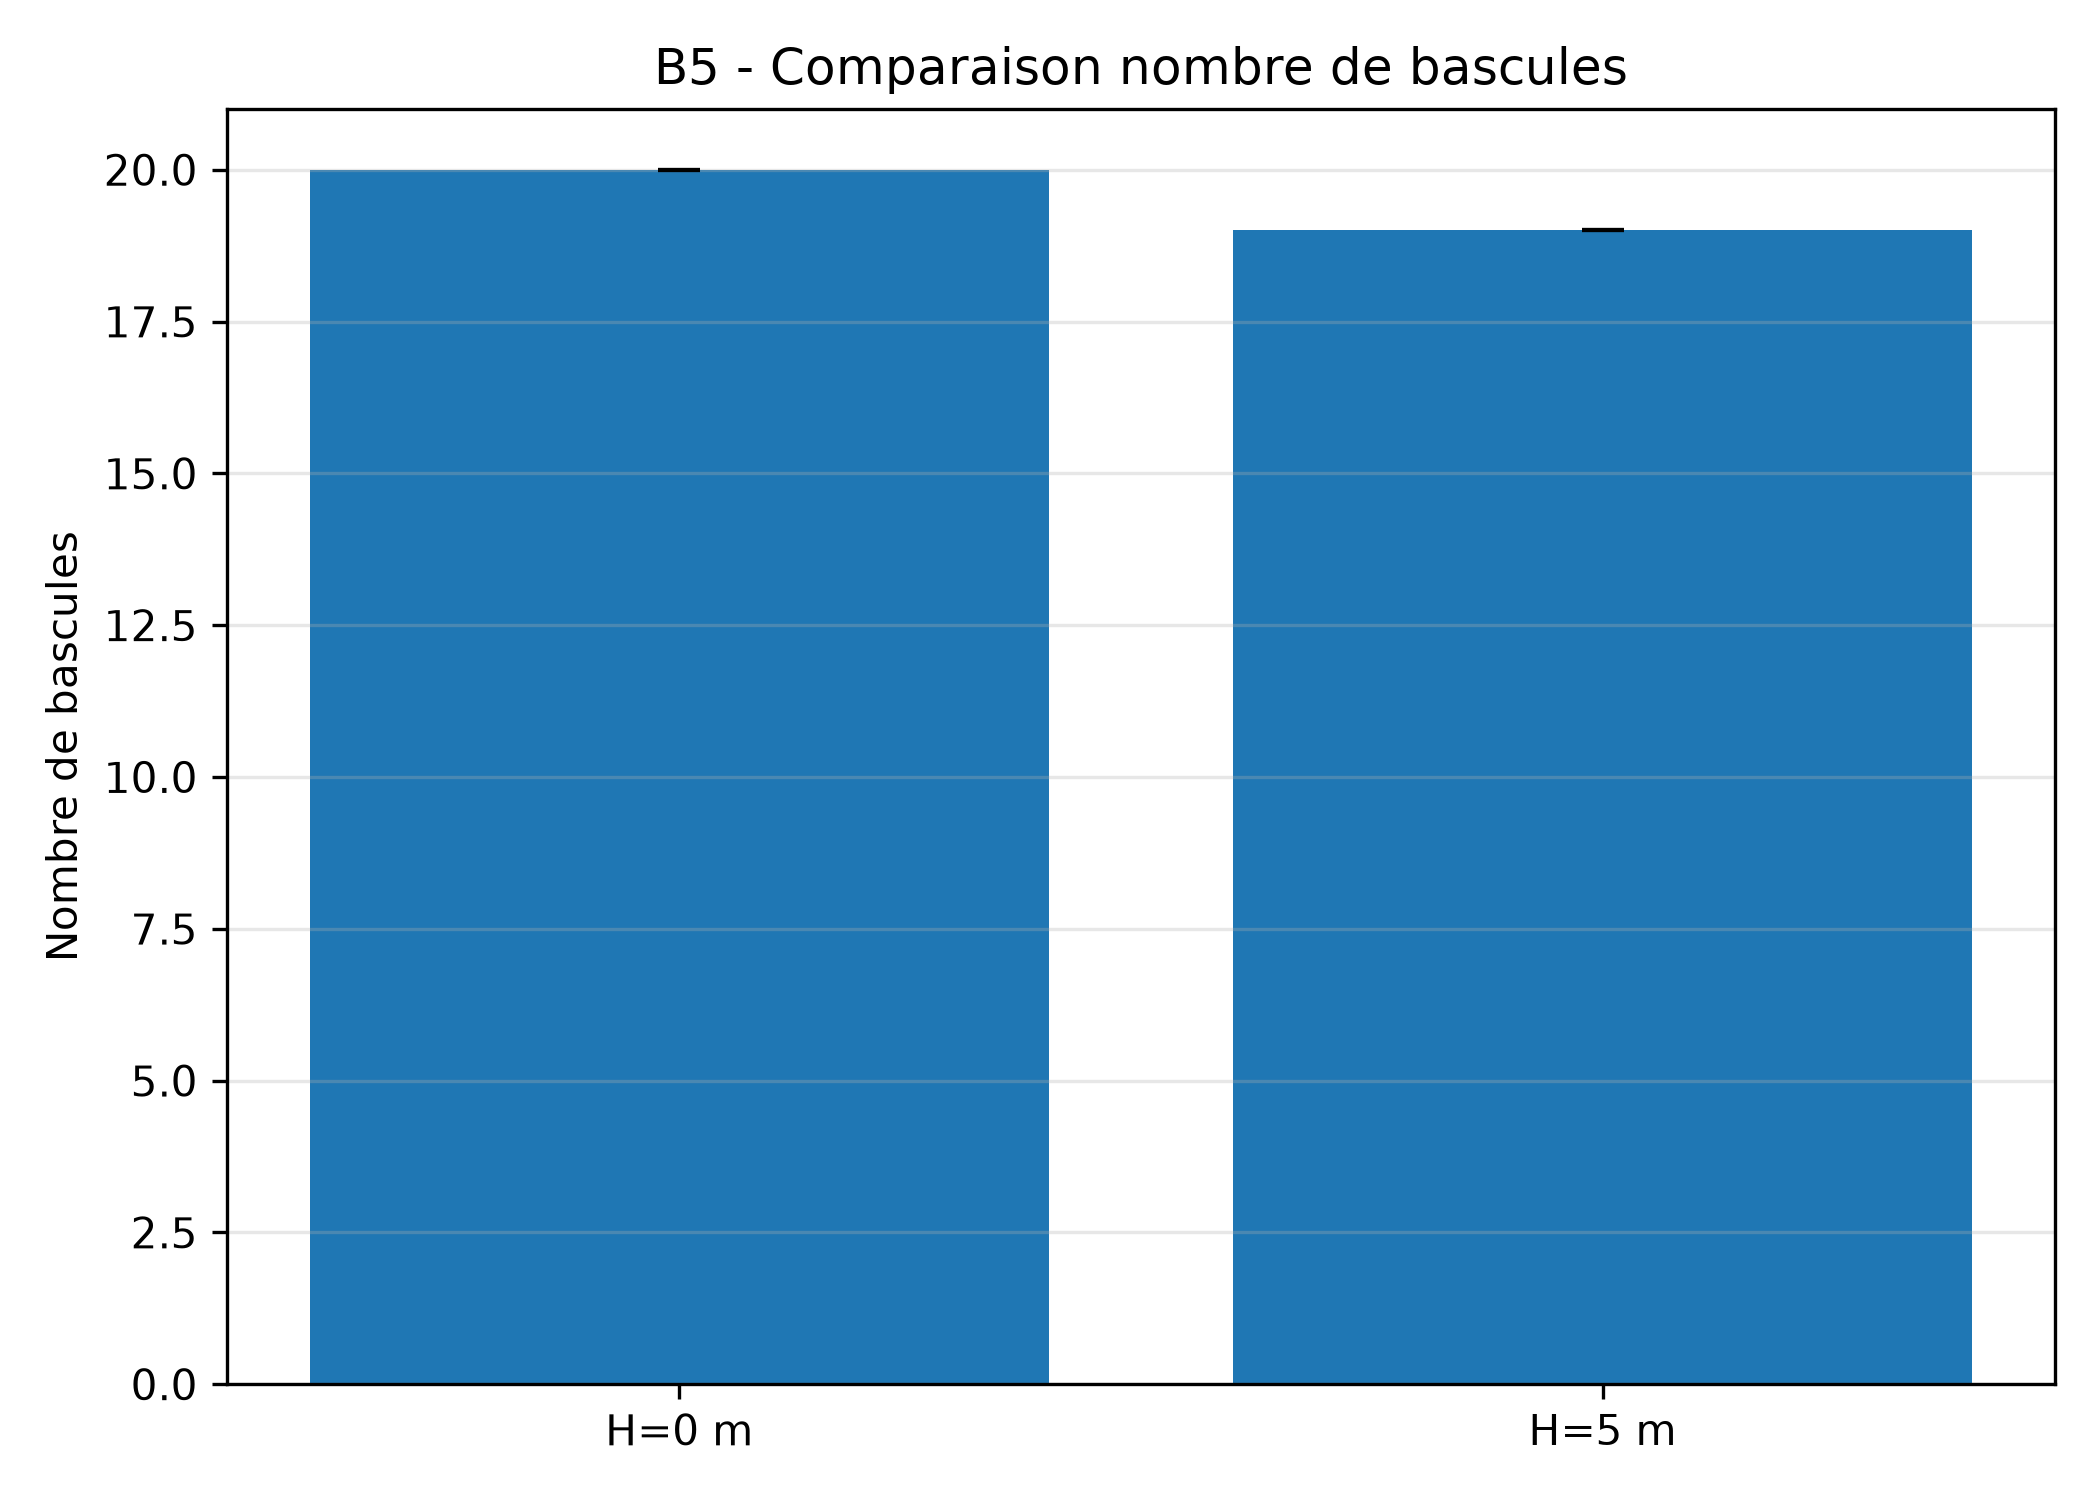
\includegraphics[width=0.85\textwidth]
    {img/B/B5_switches.png}
    \caption{Comparaison du nombre de bascules avec et sans hystérésis.}
    \label{fig:b5_switches}
\end{figure}

\subsubsection{Effet sur les événements de ping-pong}

Le nombre d'événements de ping-pong passe de 19 sans
hystérésis à 18 avec hystérésis.

La réduction relative est :

\begin{equation}
    \frac{19-18}{19}\times100
    \approx 5,26\%
\end{equation}

Cette diminution confirme que l'hystérésis réduit
légèrement les changements d'interface rapprochés.

Cependant, la différence reste limitée dans le
scénario étudié.

% Figure 2 : Evénements de ping-pong
\begin{figure}[H]
    \centering
    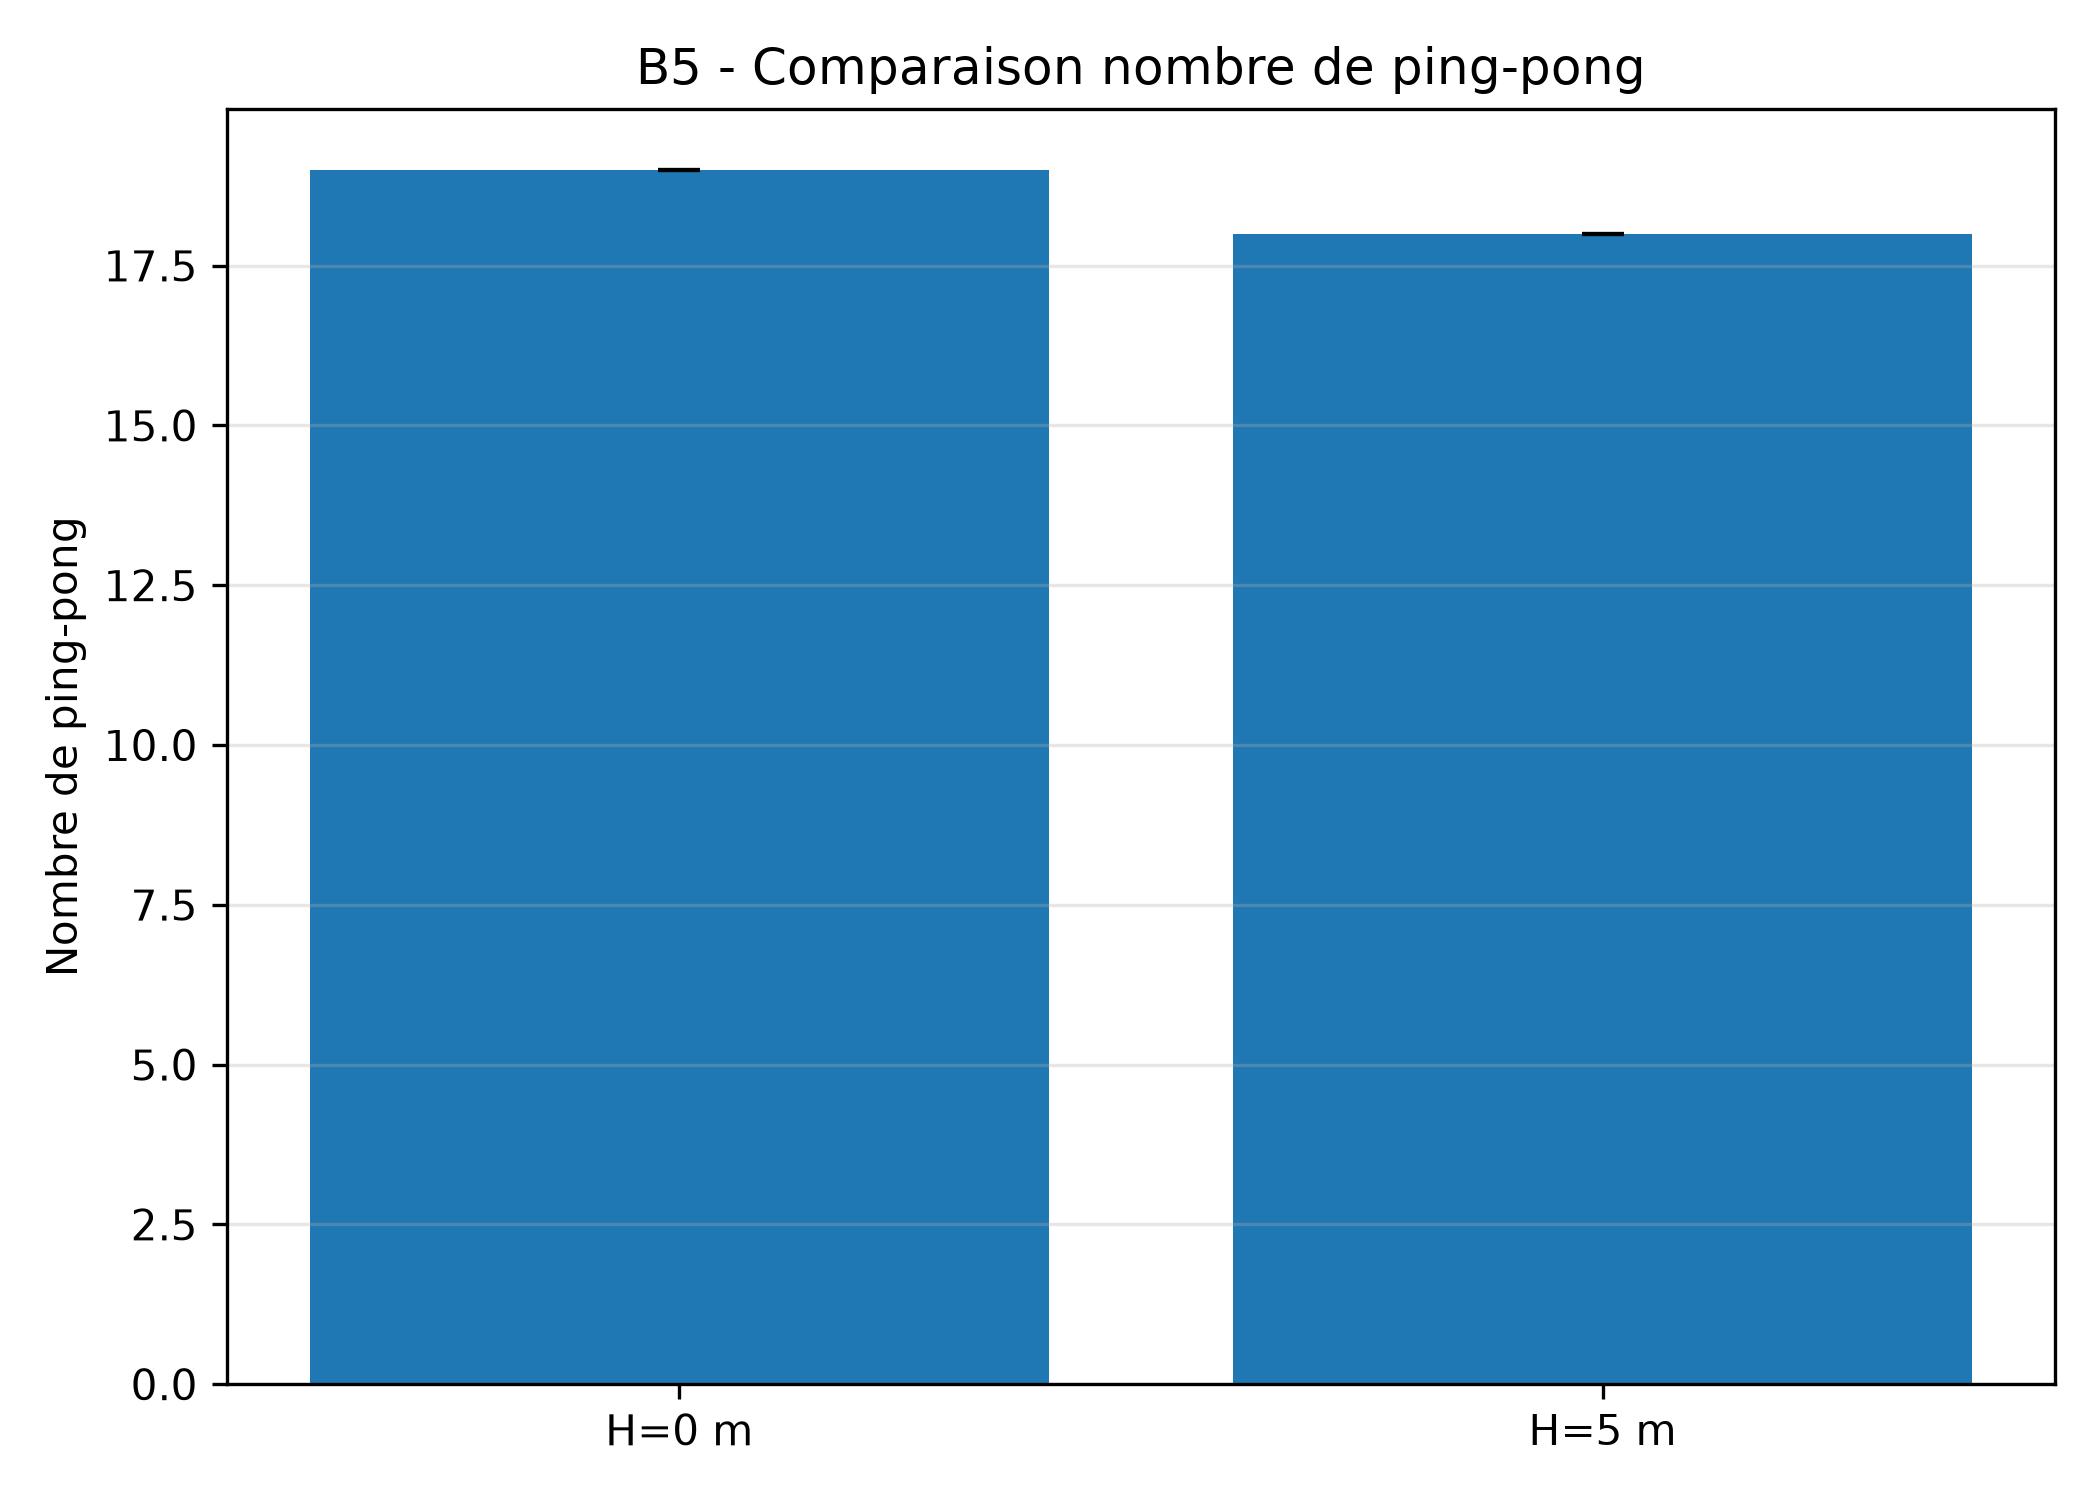
\includegraphics[width=0.85\textwidth]
    {img/B/B5_pingpong.png}
    \caption{Comparaison du nombre d'événements de ping-pong.}
    \label{fig:b5_pingpong}
\end{figure}

\subsubsection{Effet sur la stabilité du débit}

Le débit moyen reste identique dans les deux
configurations :

\begin{equation}
    \overline{D}_{H=0}
    =
    \overline{D}_{H=5}
    =
    2\ \mathrm{Mbps}
\end{equation}

Le coefficient de variation passe de 0,00844 à 0,00846.

Cette légère augmentation indique que la dispersion
relative du débit n'a pas diminué avec l'introduction
de l'hystérésis. La différence observée reste toutefois
très faible et ne permet pas de conclure à une
dégradation significative de la stabilité.

Ainsi, dans cette configuration, l'hystérésis réduit
légèrement le nombre de bascules, mais ne produit pas
d'amélioration mesurable de la stabilité du débit.

% Figure 3 : Coefficient de variation du débit
\begin{figure}[H]
    \centering
    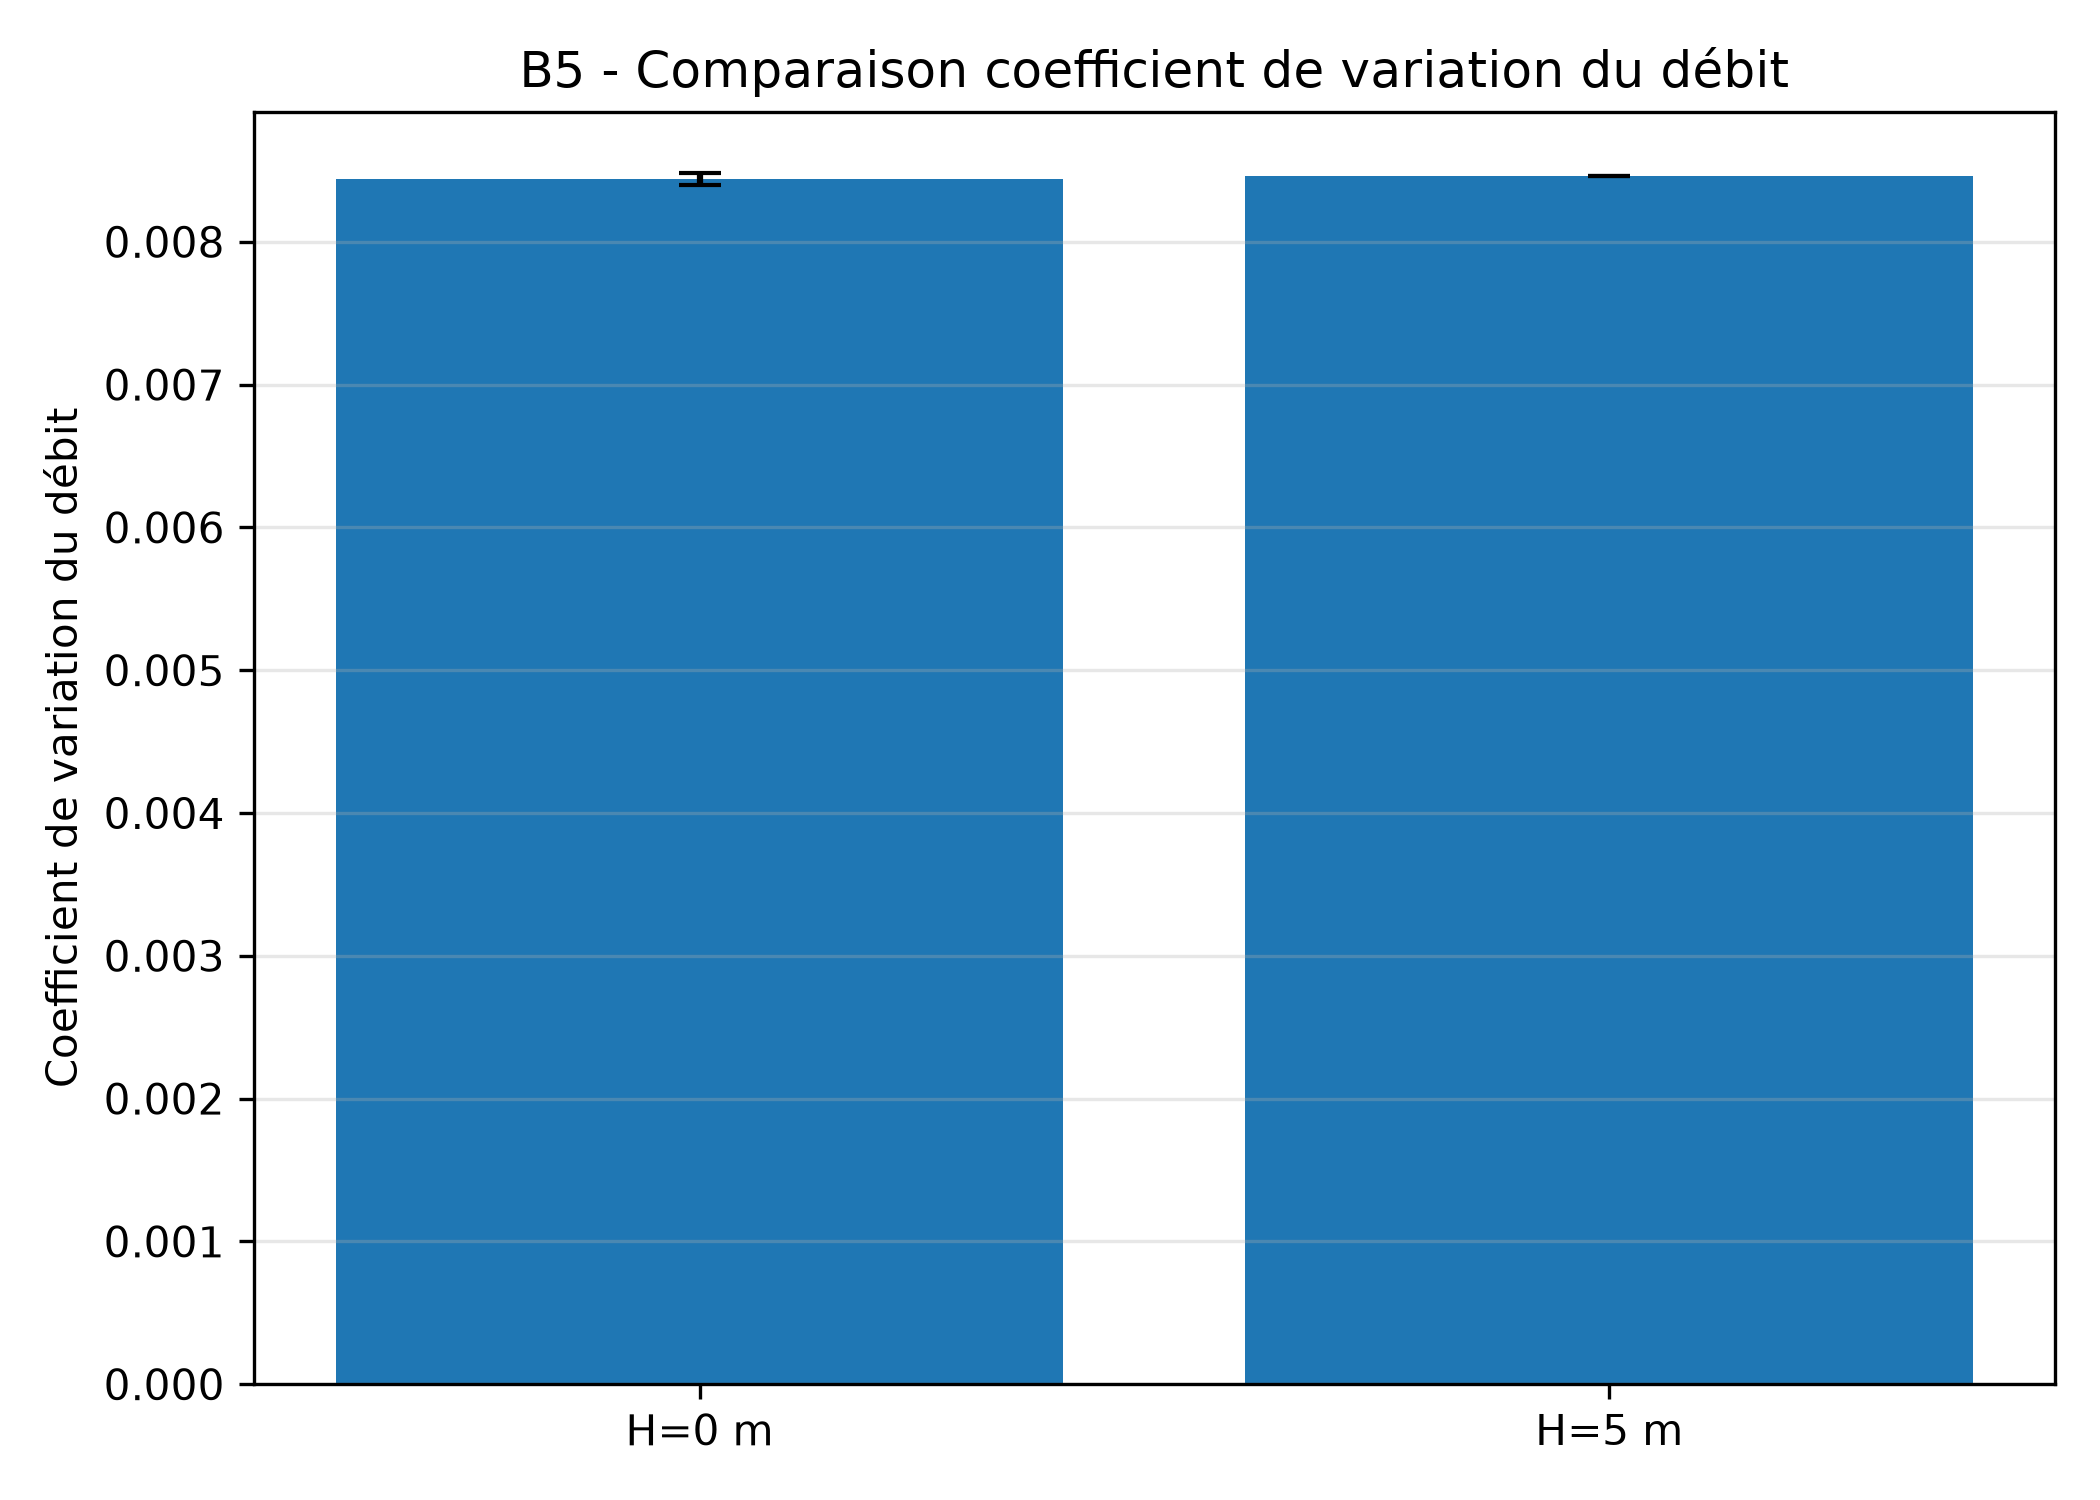
\includegraphics[width=0.85\textwidth]
    {img/B/B5_throughput_cv.png}
    \caption{Comparaison du coefficient de variation du débit reçu.}
    \label{fig:b5_cv}
\end{figure}

\subsubsection{Effet sur le trafic et les performances}

La proportion du volume reçu via Wi-Fi diminue
légèrement, passant de 51,28 \% à 50 \%.

Cette différence est cohérente avec le fait que l'UE
entre plus tard dans la couverture Wi-Fi et la quitte
plus tôt lorsque l'hystérésis est activée.

Le débit moyen reste égal au débit nominal de 2 Mbps
dans les deux configurations. Aucun paquet perdu ni
aucune interruption de service mesurée n'ont été
observés dans ces exécutions.

Le délai moyen augmente légèrement, passant de
9,184 ms à 9,397 ms, tandis que le délai maximal
reste identique à 22,731 ms.

% Figure 4 : Proportion du volume reçu via Wi-Fi
\begin{figure}[H]
    \centering
    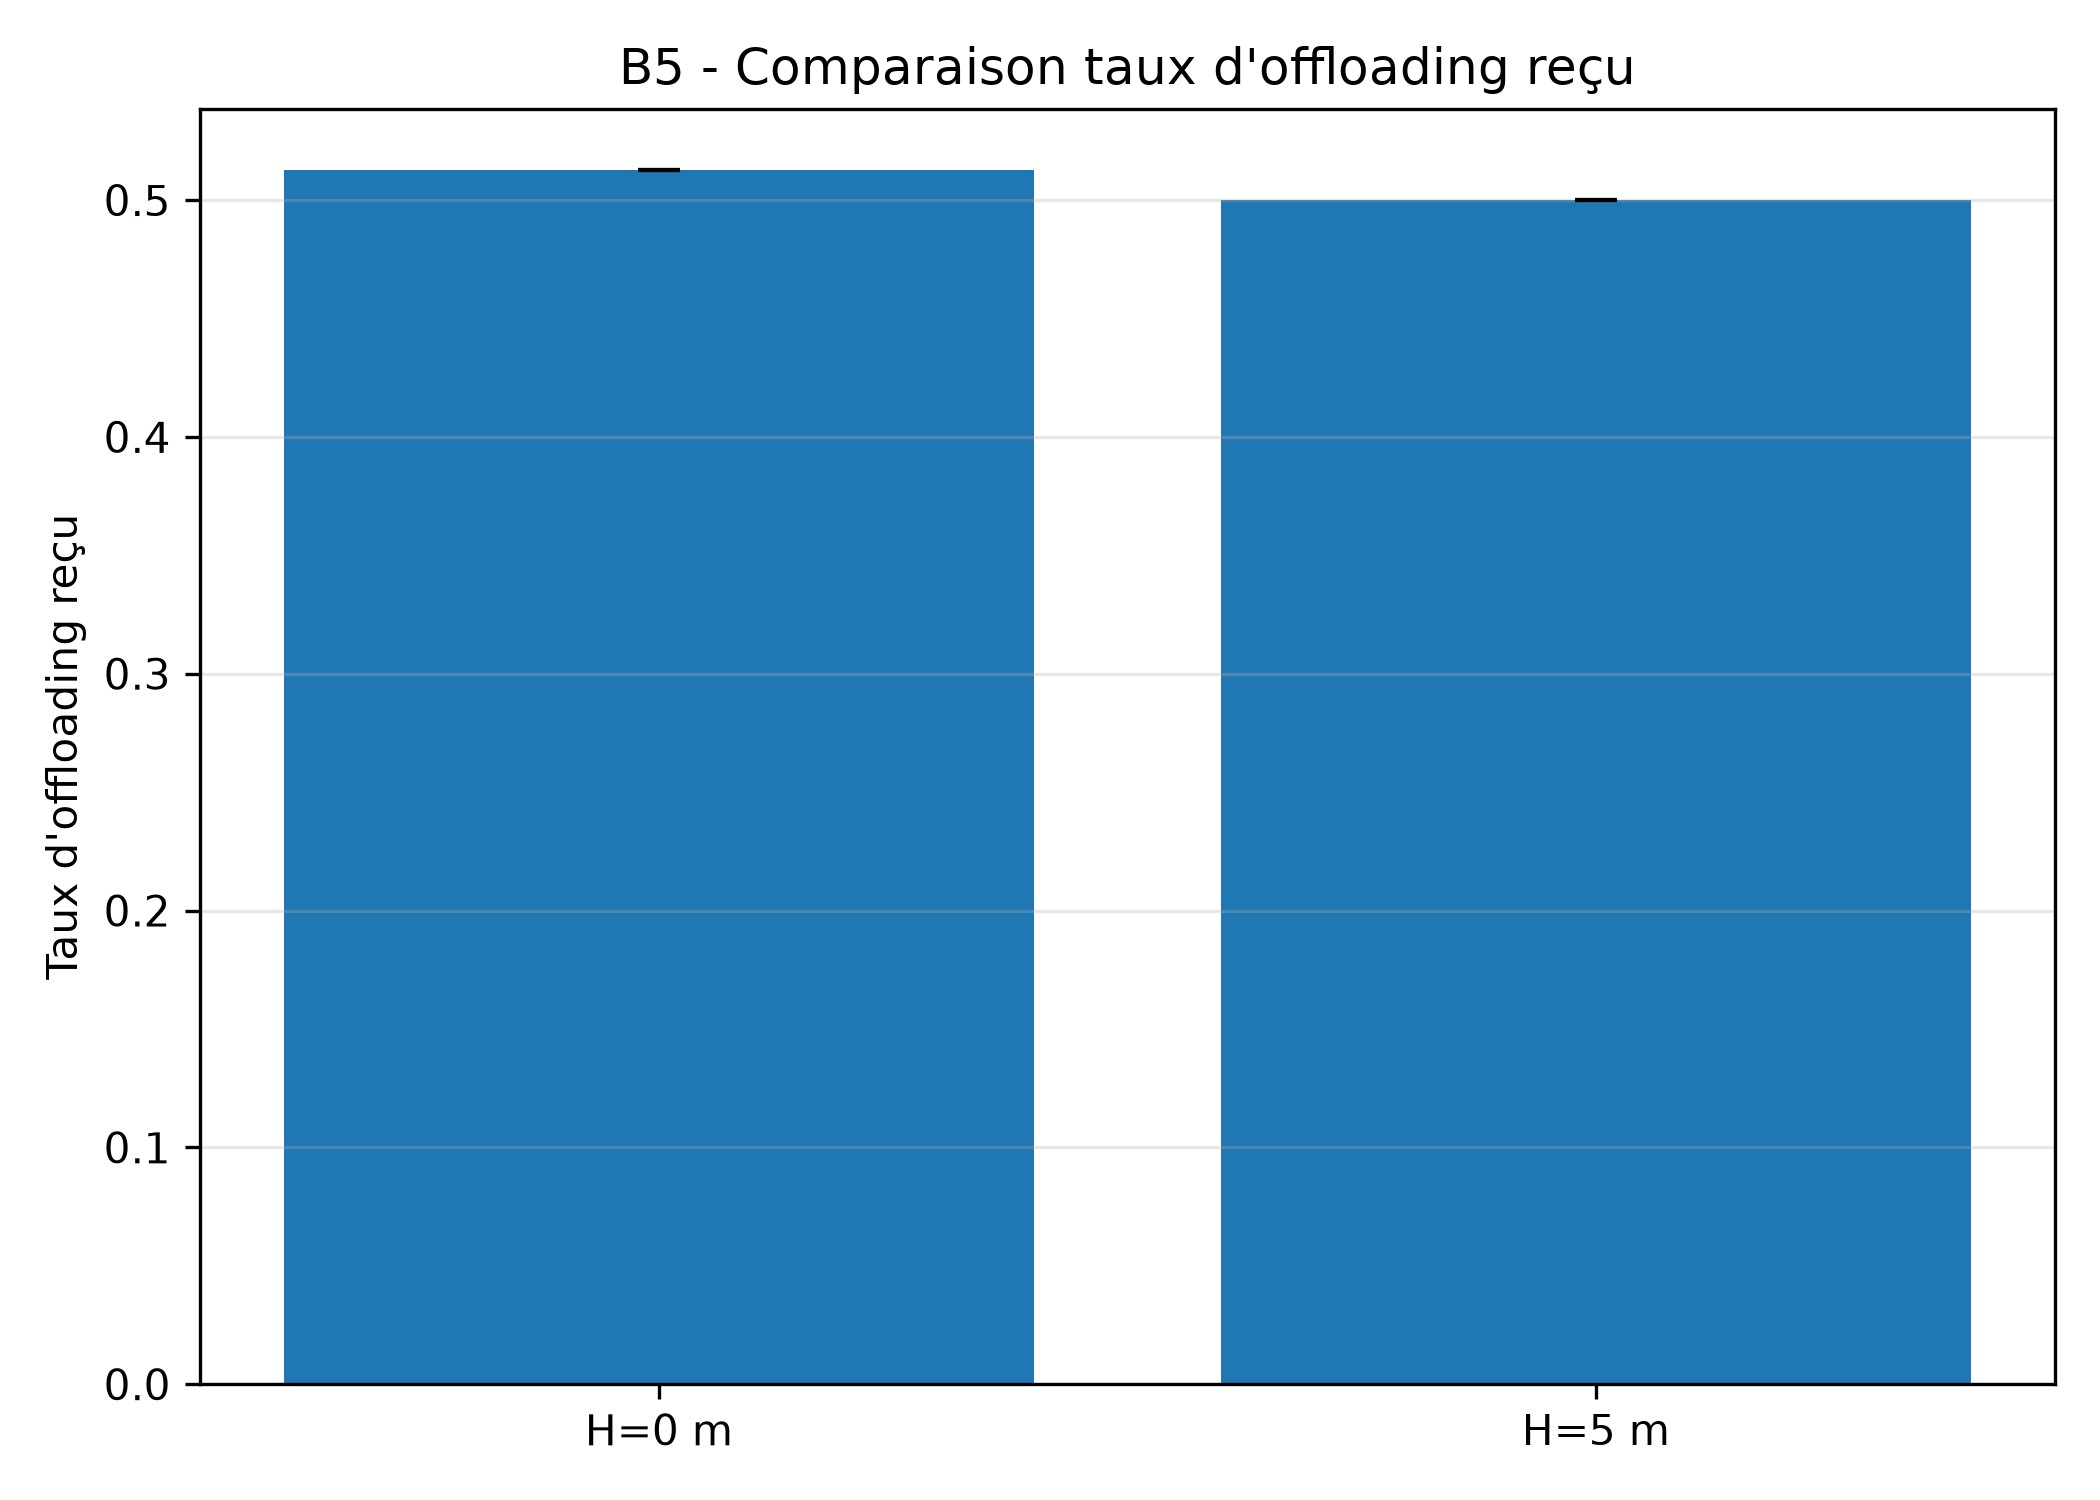
\includegraphics[width=0.85\textwidth]
    {img/B/B5_offloading.png}
    \caption{Comparaison de la proportion du volume reçu via Wi-Fi.}
    \label{fig:b5_offloading}
\end{figure}

\subsection{Discussion des résultats}

Les résultats montrent que l'introduction d'une
hystérésis permet de réduire le nombre de changements
d'interface lorsque l'UE se déplace à proximité de la
limite de couverture Wi-Fi.

Néanmoins, l'amélioration observée reste modeste :
le nombre total de bascules diminue de 5 \%, tandis
que le nombre d'événements de ping-pong diminue
d'environ 5,26 \%.

Par ailleurs, le coefficient de variation du débit
reste pratiquement identique entre les deux
configurations. L'hystérésis n'apporte donc pas,
dans ce scénario, de gain significatif en matière
de stabilité du débit.

Il faut également préciser que les cinq exécutions
utilisent la même graine initiale et que le shadowing
ainsi que le bruit sur la distance sont désactivés.
Les écarts-types nuls obtenus pour le nombre de
bascules et les événements de ping-pong traduisent
donc essentiellement la reproductibilité du scénario
déterministe. Ces exécutions ne constituent pas une
étude de la variabilité inter-graines.

\subsection{Conclusion}

Cette expérience a permis d'étudier l'influence de
l'hystérésis sur le mécanisme de bascule entre LTE
et Wi-Fi.

En introduisant deux seuils distincts, un seuil
d'entrée de 45 m et un seuil de sortie de 55 m,
le nombre moyen de bascules passe de 20 à 19,
soit une réduction de 5 \%.

Le nombre d'événements de ping-pong diminue
également, tandis que le débit moyen reste stable
à 2 Mbps. Cependant, le coefficient de variation
ne montre aucune amélioration notable de la
stabilité du débit.

Nous pouvons donc conclure que l'hystérésis
constitue un mécanisme pertinent pour limiter
les bascules répétées à proximité de la limite
de couverture, mais que son efficacité dépend
du scénario de mobilité et des paramètres choisis.
Dans le scénario étudié, son apport est réel
mais limité.

% ============================================================
% FIN DE LA QUESTION B5
% ============================================================

\section{Question 8 : Critère de bascule orienté réseau (décision côté PGW)}
% ---------------------------------------------------------------------

\subsection{Objectif}
Les questions précédentes étudient un critère \emph{orienté terminal} : c'est
l'UE qui mesure sa distance (ou son RSSI) et qui modifie sa table de routage.
La question B8 implémente l'approche duale, inspirée des architectures
d'offloading pilotées par le c\oe ur de réseau (PGW/ANDSF) : la décision est
prise \emph{par flux applicatif}, selon le protocole de transport et le débit,
indépendamment de la position de l'UE.

\subsection{Principe de décision}
NS-3 ne modélise ni l'ANDSF ni le PCRF. Le rôle du PGW est donc simulé par une
fonction exécutée \emph{une seule fois par flux}, avant le démarrage du trafic.
La règle appliquée est celle de l'énoncé :
\[
\text{Wi-Fi} \iff (\text{protocole} = \text{UDP}) \;\wedge\; (D_{\text{flux}} > D_{\text{seuil}}),
\qquad D_{\text{seuil}} = 1~\text{Mb/s},
\]
et LTE dans tous les autres cas. Ainsi, un flux UDP à débit élevé est déchargé
vers le Wi-Fi, tandis qu'un flux TCP reste sur LTE, où l'EPC garantit
l'ordonnancement et la qualité de service.

\begin{lstlisting}[language=C++]
static bool PolicyOffloadToWifi(bool isUdp, double rateMbps, double thrMbps)
{
    return isUdp && rateMbps > thrMbps;   // UDP au-dessus du seuil -> Wi-Fi
}
\end{lstlisting}

\begin{figure}[H]
      \centering
      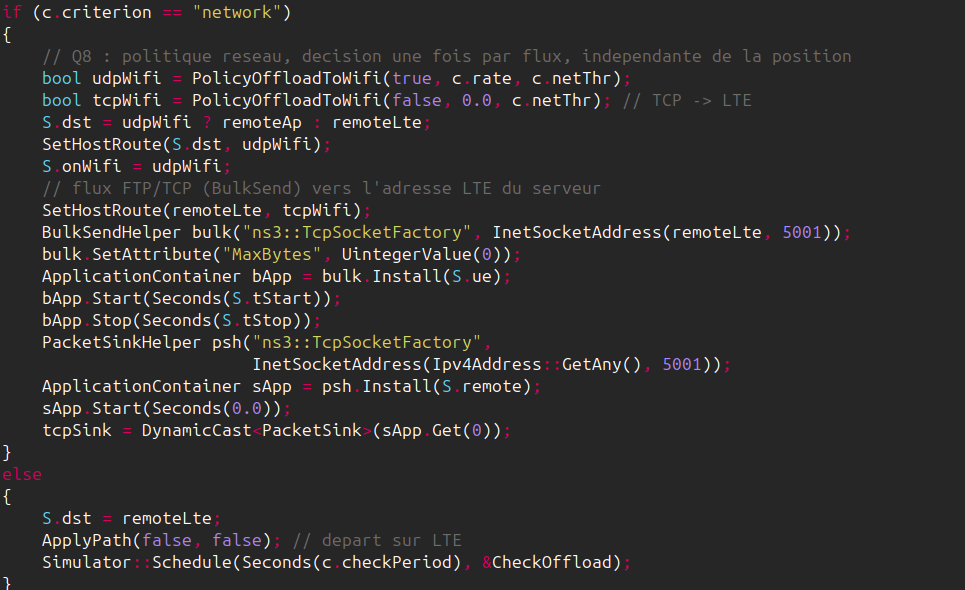
\includegraphics[width=0.7\textwidth]{img/C/pic0_criterion.png}
      \caption{Capture de la Configuration des modes }
\end{figure}

\subsection{Scénario et paramètres}
Le scénario de la question B1 est repris (un eNodeB, un point d'accès Wi-Fi
802.11n, un UE à double interface, un serveur distant). Deux flux
\emph{simultanés} sont émis de l'UE vers le serveur (sens montant) :

\begin{itemize}
  \item un flux \textbf{UDP CBR} de 2~Mb/s (paquets de 1200 octets, port 9000),
        supérieur au seuil de 1~Mb/s : il est donc routé vers le Wi-Fi ;
  \item un flux \textbf{TCP} de type FTP (\texttt{BulkSendApplication}, port
        5001), routé vers LTE.
\end{itemize}

Le routage est réalisé par des routes \emph{hôte} statiques
(\texttt{AddHostRouteTo}) dans la table de l'UE : le flux UDP est adressé à
l'adresse Wi-Fi du serveur (10.0.2.2, joignable via l'AP), le flux TCP à son
adresse LTE (1.0.0.2, joignable via le PGW). Ces routes ne sont jamais
modifiées pendant la simulation.

\begin{table}[H]
\centering
\caption{Adressage et chemins utilisés dans la question B8}
\begin{tabular}{llll}
\toprule
Flux & Source & Destination & Chemin \\
\midrule
UDP CBR 2 Mb/s (port 9000) & 10.0.1.2 (UE, Wi-Fi) & 10.0.2.2 (serveur) & UE $\to$ AP $\to$ serveur \\
TCP bulk (port 5001)       & 7.0.0.2 (UE, LTE)    & 1.0.0.2 (serveur) & UE $\to$ eNodeB $\to$ PGW $\to$ serveur \\
\bottomrule
\end{tabular}
\end{table}

\begin{lstlisting}
                     +---- LTE path ------------------------------+
                     |                                             |
UE --(LTE radio)--> eNodeB --(S1)--> SGW/PGW --(p2p 1.0.0.0/8)--> RemoteHost
 |                                                                   ^
 +--(WiFi radio)--> AP --------(p2p 10.0.2.0/24)---------------------+
                     +---- WiFi path ----+
\end{lstlisting}

\subsection{Vérification par FlowMonitor et pcap}
La vérification a été effectuée sur une exécution de contrôle où l'UE démarre
dans la zone du hotspot (vitesse 1~m/s, durée 20~s), afin que les premiers
paquets du flux UDP puissent effectivement traverser le Wi-Fi :
\begin{lstlisting}
./ns3 run "tp3-offload --criterion=network --speed=1 --simTime=20 \
           --pcap=true --outDir=results/tp3/q8 --tag=net_proof"
\end{lstlisting}

Le fichier de synthèse de cette exécution donne : 4\,500\,000 octets émis sur
le chemin Wi-Fi et 4\,500\,000 octets reçus par le serveur via le Wi-Fi, aucune
perte, un débit moyen de 2,00~Mb/s pour le flux UDP et un débit de
1,65~Mb/s pour le flux TCP (via LTE). Aucune bascule n'est comptabilisée,
conformément au principe du critère réseau.

\begin{figure}[H]
      \centering
      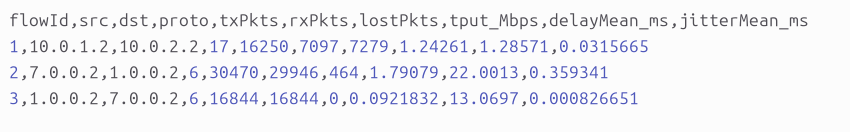
\includegraphics[width=0.7\textwidth]{img/C/pic1_flowmon.png}
      \caption{Deux flux : UDP 10.0.1.2 $\to$ 10.0.2.2 et TCP 7.0.0.2 $\to$ 1.0.0.2}
\end{figure}


\paragraph{Capture Wireshark.}
Les captures pcap sont ouvertes dans Wireshark :
\begin{itemize}
  \item sur la liaison AP--serveur (\texttt{*\_remote-ap*.pcap}), avec le filtre
        \texttt{udp.port == 9000}, on observe le flux UDP dès son premier
        paquet ; aucun segment TCP n'y figure ;
  \item sur la liaison PGW--serveur (\texttt{*\_remote-lte*.pcap}), avec le
        filtre \texttt{tcp.port == 5001}, on observe le flux TCP, et
        \emph{aucun} paquet UDP de port 9000.
\end{itemize}

\begin{figure}[H]
      \centering
      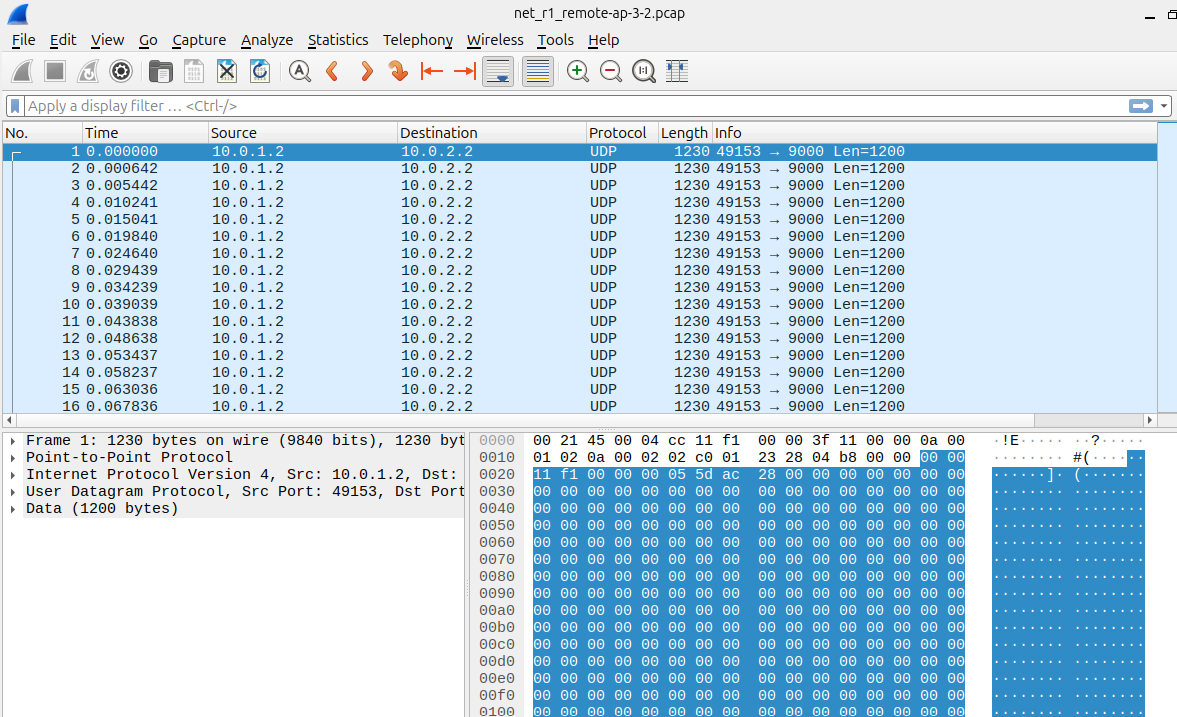
\includegraphics[width=0.7\textwidth]{img/C/pic2_udp_flow.png}
      \caption{flux des paquets UDP de l'adresse source 10.0.1.2}
\end{figure}

\begin{figure}[H]
      \centering
      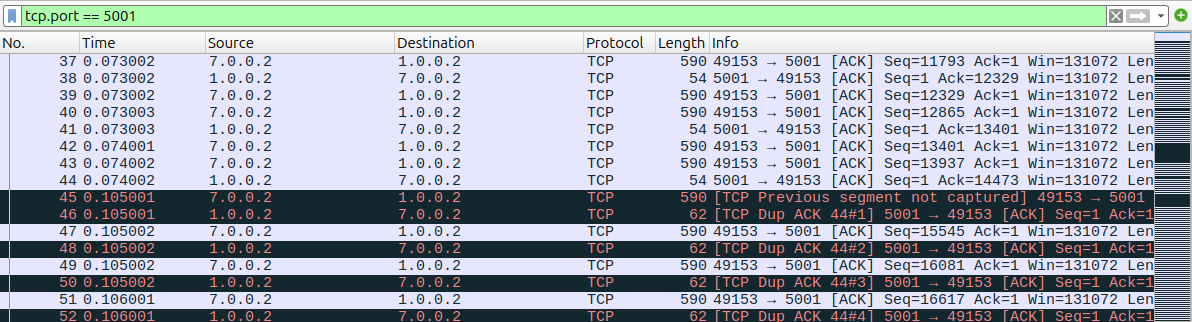
\includegraphics[width=0.7\textwidth]{img/C/pic3_tcp.png}
      \caption{le handshake TCP SYN/SYN-ACK dès t $\approx$ 1 s et l'absence de trafic UDP 9000}
\end{figure}

\subsection{Limites de la modélisation}
\begin{itemize}
  \item La fonction de politique est exécutée dans la simulation et agit sur la
        table de routage de l'UE : le PGW n'est pas une entité décisionnelle
        distincte, conformément à la simplification demandée par l'énoncé.
  \item La décision est statique : elle est prise au démarrage de chaque flux
        et n'est pas réévaluée en cours de route.
  \item Les flux sont émis dans le sens montant ; en sens descendant, le choix
        du chemin relèverait de la table de routage du serveur.
\end{itemize}

\subsection{Conclusion de B8}
La politique orientée réseau fonctionne comme attendu : le flux UDP à 2~Mb/s
emprunte le Wi-Fi dès son premier paquet et le flux TCP reste sur LTE, ce qui
est confirmé par FlowMonitor et par les captures pcap. Le comportement de ce
critère en situation de mobilité est étudié à la question B9.

% ---------------------------------------------------------------------
\section{Question 9 : Comparaison des critères orienté terminal et orienté réseau}
% ---------------------------------------------------------------------

\subsection{Protocole expérimental}
Les trois configurations suivantes sont comparées sur la \emph{même
trajectoire} et les \emph{mêmes graines} :
\begin{itemize}
  \item \texttt{dist\_h0} : critère terminal à seuil de distance unique ($H=0$) ;
  \item \texttt{dist\_h5} : critère terminal avec hystérésis ($H=5$~m, seuils
        d'entrée et de sortie à 45~m et 55~m) ;
  \item \texttt{net} : critère réseau de la question B8.
\end{itemize}

\begin{table}[H]
\centering
\caption{Paramètres de la campagne de la question B9}
\begin{tabular}{ll}
\toprule
Paramètre & Valeur \\
\midrule
Rayon nominal du hotspot $R$ & 50 m \\
Trajectoire & ligne droite traversant l'AP (\texttt{line}) \\
Vitesse de l'UE & 5 m/s \\
Durée de simulation & 80 s (trafic de 1 s à 79 s) \\
Débit CBR UDP & 2 Mb/s (paquets de 1200 octets) \\
Décalage latéral aléatoire & $b \sim \mathcal{U}(0,\,0{,}5\,R)$ (\texttt{offsetFrac}=0,5) \\
Bruit de mesure de distance (critères terminal) & $\sigma_d = 3$ m (\texttt{distNoise}=3) \\
Shadowing & désactivé (\texttt{shadowSigma}=0) \\
Période de vérification du critère & 0,5 s \\
Fenêtre de détection du ping-pong & 15 s (valeur par défaut du code) \\
Graine / numéros de run & graine = 1 / runs 1 à 5 \\
Nombre de simulations & $3 \times 5 = 15$ \\
\bottomrule
\end{tabular}
\end{table}

Le décalage latéral $b$ est tiré avec la même graine pour les trois
configurations : à numéro de run égal, les trois critères parcourent donc
exactement la même trajectoire (valeur de \texttt{offset\_b} identique dans
les fichiers de synthèse). Les moyennes sont accompagnées de l'écart-type
expérimental (correction de Bessel).

\paragraph{Définition de l'interruption.}
La définition de la question B4 est reprise : une interruption est une durée
pendant laquelle le débit reçu tombe sous 50\,\% du débit nominal. Dans cette
campagne, elle est évaluée sur des intervalles \emph{fixes} de 100~ms (et non
sur une fenêtre glissante) autour de chaque bascule, avec le nombre de
paquets perdus et le pic de délai sur cette fenêtre. La résolution temporelle
est donc de 100~ms. Pour le critère réseau, aucune bascule n'a lieu en cours
de flux : l'interruption \emph{par bascule} est sans objet (N/A).

\subsection{Résultats}

\begin{table}[H]
\centering
\caption{Commutations, offloading et interruption (moyenne $\pm$ écart-type sur 5 runs)}
\small
\begin{tabular}{lccccc}
\toprule
Config. & Bascules & Ping-pong & Offloading & Interruption & Pic de délai \\
        &          &           & effectif$^{(a)}$ & par bascule (s) & (ms) \\
\midrule
\texttt{dist\_h0} & $3{,}20 \pm 1{,}10$ & $1{,}20 \pm 1{,}10$ & $0{,}24 \pm 0{,}01$ & $0{,}00 \pm 0{,}00$ & $21{,}07 \pm 2{,}20$ \\
\texttt{dist\_h5} & $2{,}00 \pm 0{,}00$ & $0{,}00 \pm 0{,}00$ & $0{,}25 \pm 0{,}02$ & $0{,}00 \pm 0{,}00$ & $20{,}23 \pm 2{,}43$ \\
\texttt{net}      & $0{,}00 \pm 0{,}00$ & $0{,}00 \pm 0{,}00$ & $\approx 0{,}43$ $^{(b)}$ & N/A & N/A \\
\bottomrule
\end{tabular}

\smallskip
\begin{minipage}{0.92\textwidth}\footnotesize
$^{(a)}$ Fraction des octets \emph{reçus par le serveur via le Wi-Fi}.\\
$^{(b)}$ Le fichier de synthèse affiche 1,00 pour \texttt{net}, car seuls les
octets \emph{reçus} sont comptés et tous sont passés par le Wi-Fi. Rapporté au
volume \emph{émis}, l'offloading effectif vaut $1 - 0{,}5704 \approx 0{,}43$.
(sur le run 1, des paquets sont encore reçus via le Wi-Fi jusqu'à
85,5~m de l'AP, soit un rayon effectif d'environ 85~m).
\end{minipage}
\end{table}

\begin{table}[H]
\centering
\caption{Qualité de service (moyenne $\pm$ écart-type sur 5 runs)}
\small
\begin{tabular}{lcccc}
\toprule
Config. & Perte (\%) & Délai moyen (ms) & Durée sous le seuil (s) & Débit moyen (Mb/s) \\
\midrule
\texttt{dist\_h0} & $0{,}00 \pm 0{,}00$ & $13{,}58 \pm 0{,}20$ & $0{,}00 \pm 0{,}00$ & $2{,}00 \pm 0{,}00$ \\
\texttt{dist\_h5} & $0{,}00 \pm 0{,}00$ & $13{,}52 \pm 0{,}28$ & $0{,}00 \pm 0{,}00$ & $2{,}00 \pm 0{,}00$ \\
\texttt{net}      & $57{,}04 \pm 0{,}59$ & $1{,}29 \pm 0{,}01$ & $44{,}48 \pm 0{,}44$ & $0{,}86 \pm 0{,}01$ \\
\bottomrule
\end{tabular}

\smallskip
\begin{minipage}{0.92\textwidth}\footnotesize
La durée sous le seuil est cumulée sur toute la simulation (sur 78 s de
trafic), et non par bascule. Le délai moyen de \texttt{net} ne porte que sur
les paquets effectivement livrés, tous par le Wi-Fi.
\end{minipage}
\end{table}

\begin{figure}[H]
      \centering
      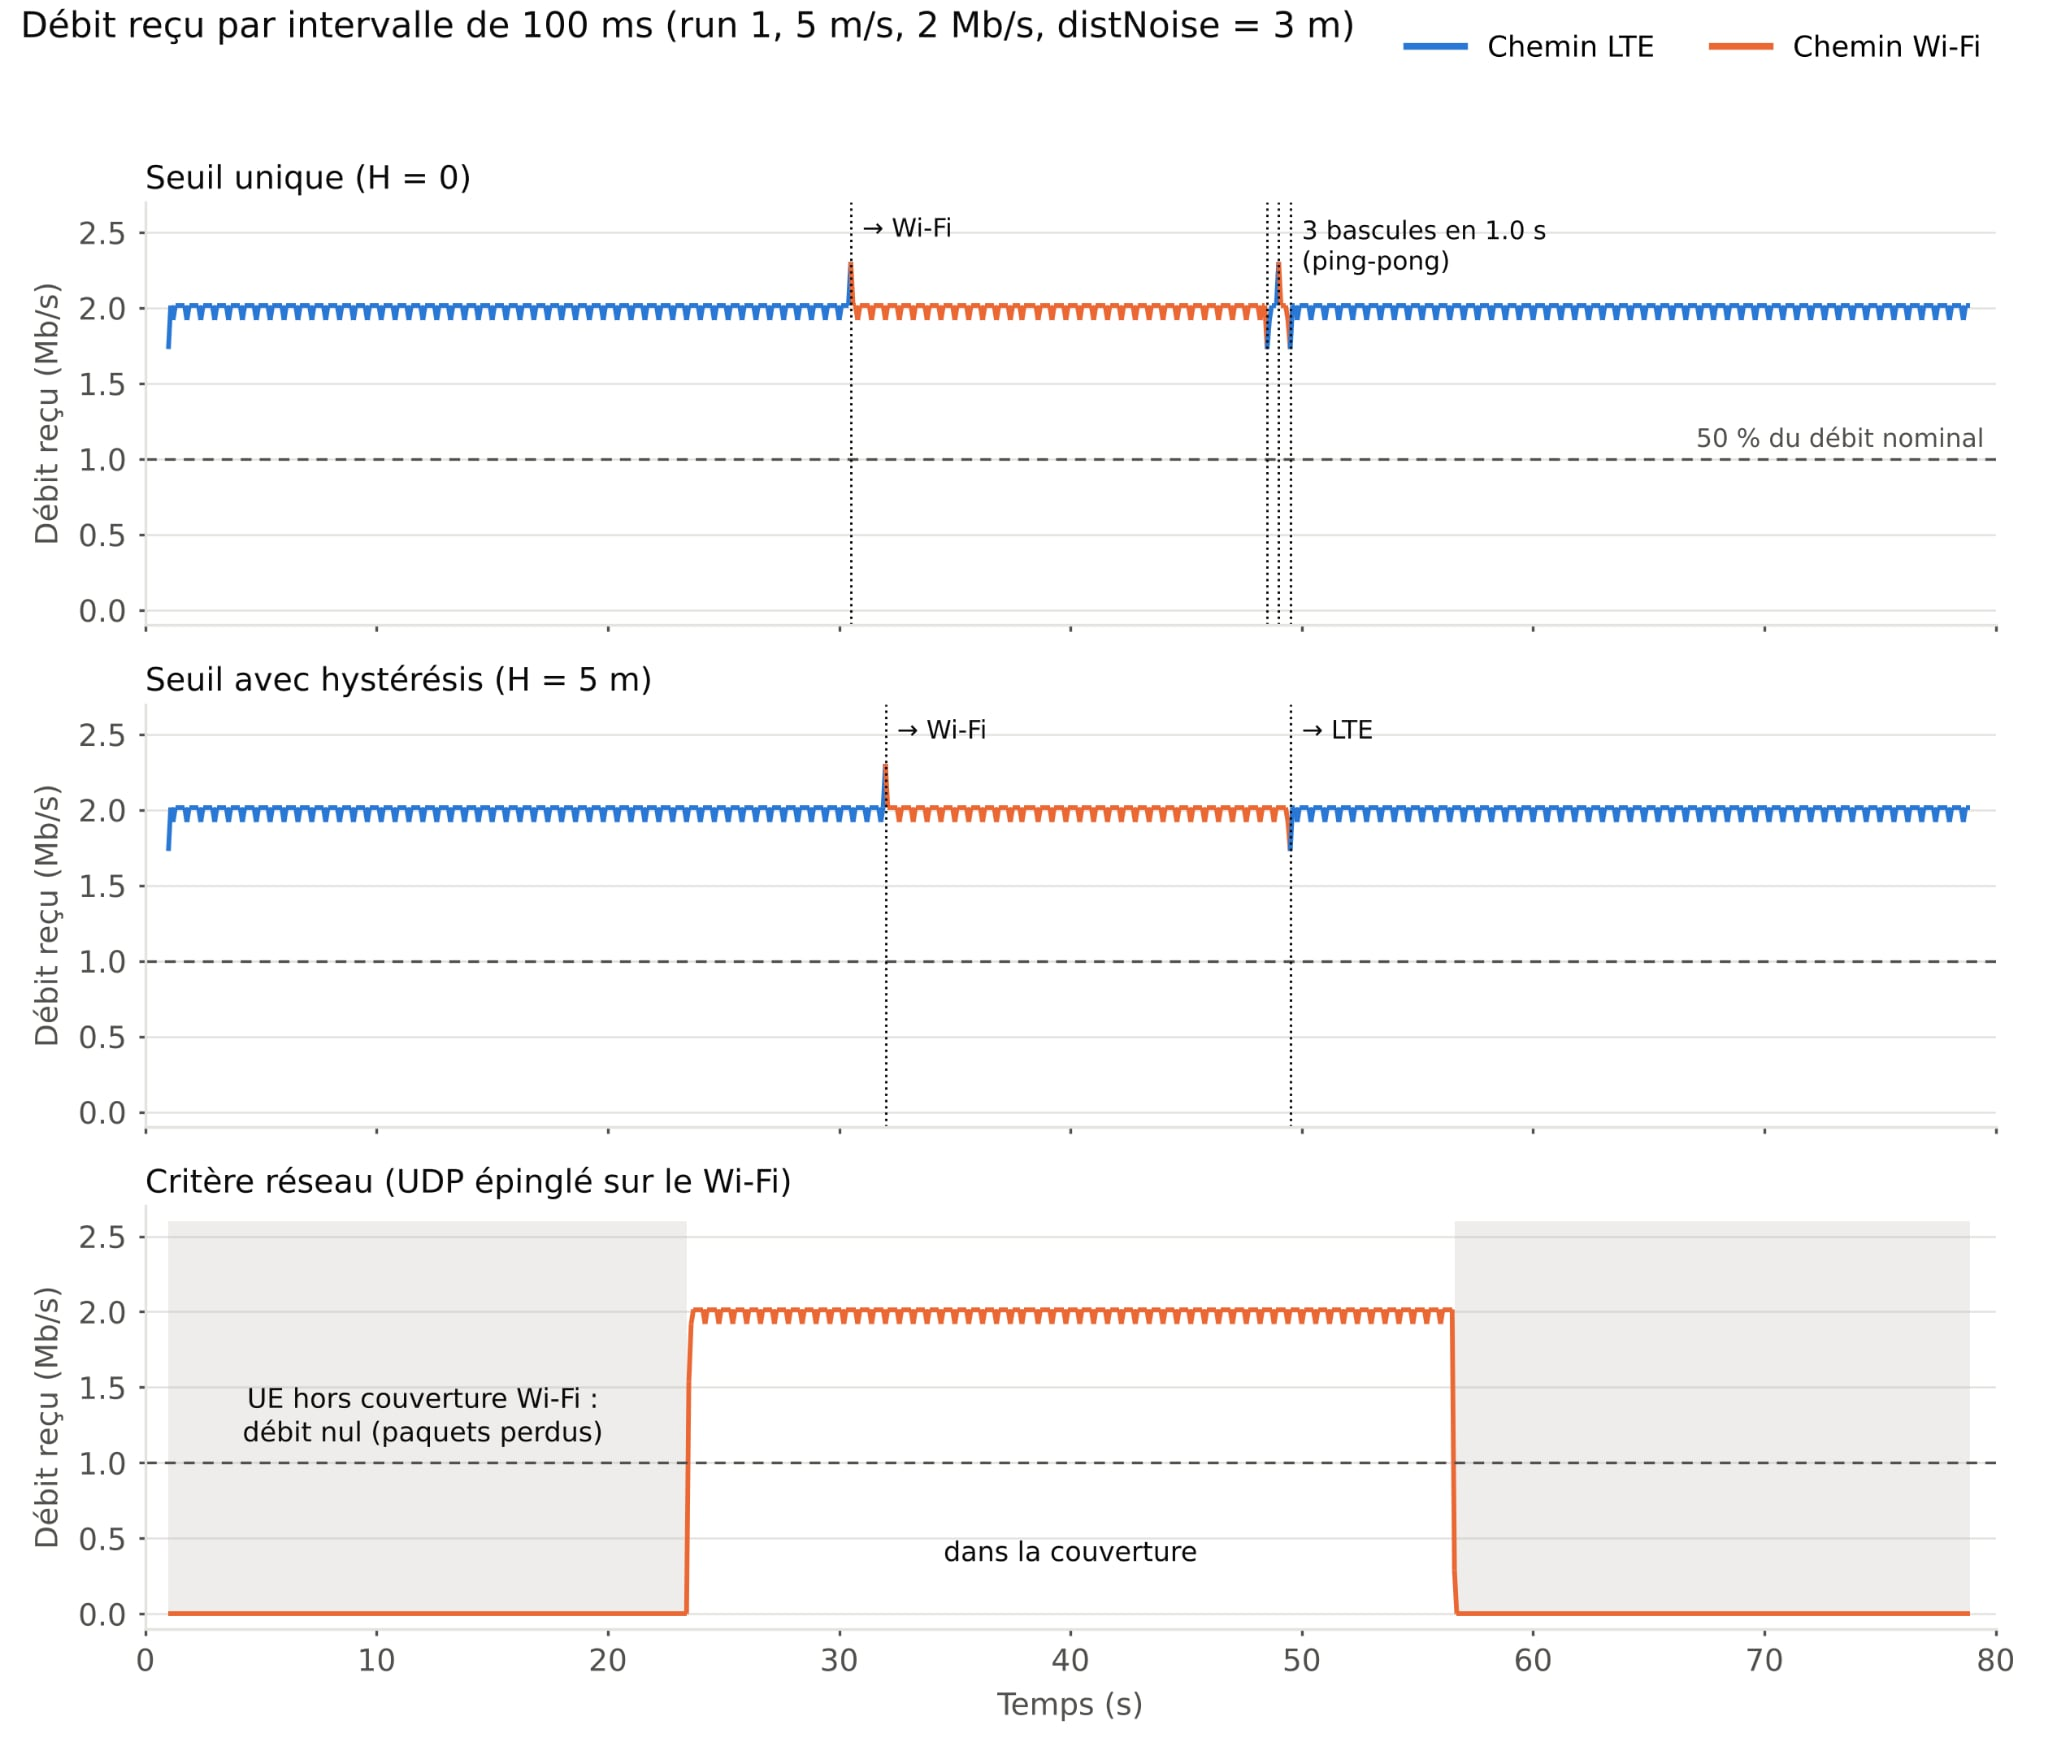
\includegraphics[width=0.7\textwidth]{img/C/pic4_debitudp.jpg}
      \caption{Nombre de bascules et taux d'offloading par critère}
\end{figure}
\begin{figure}[H]
      \centering
      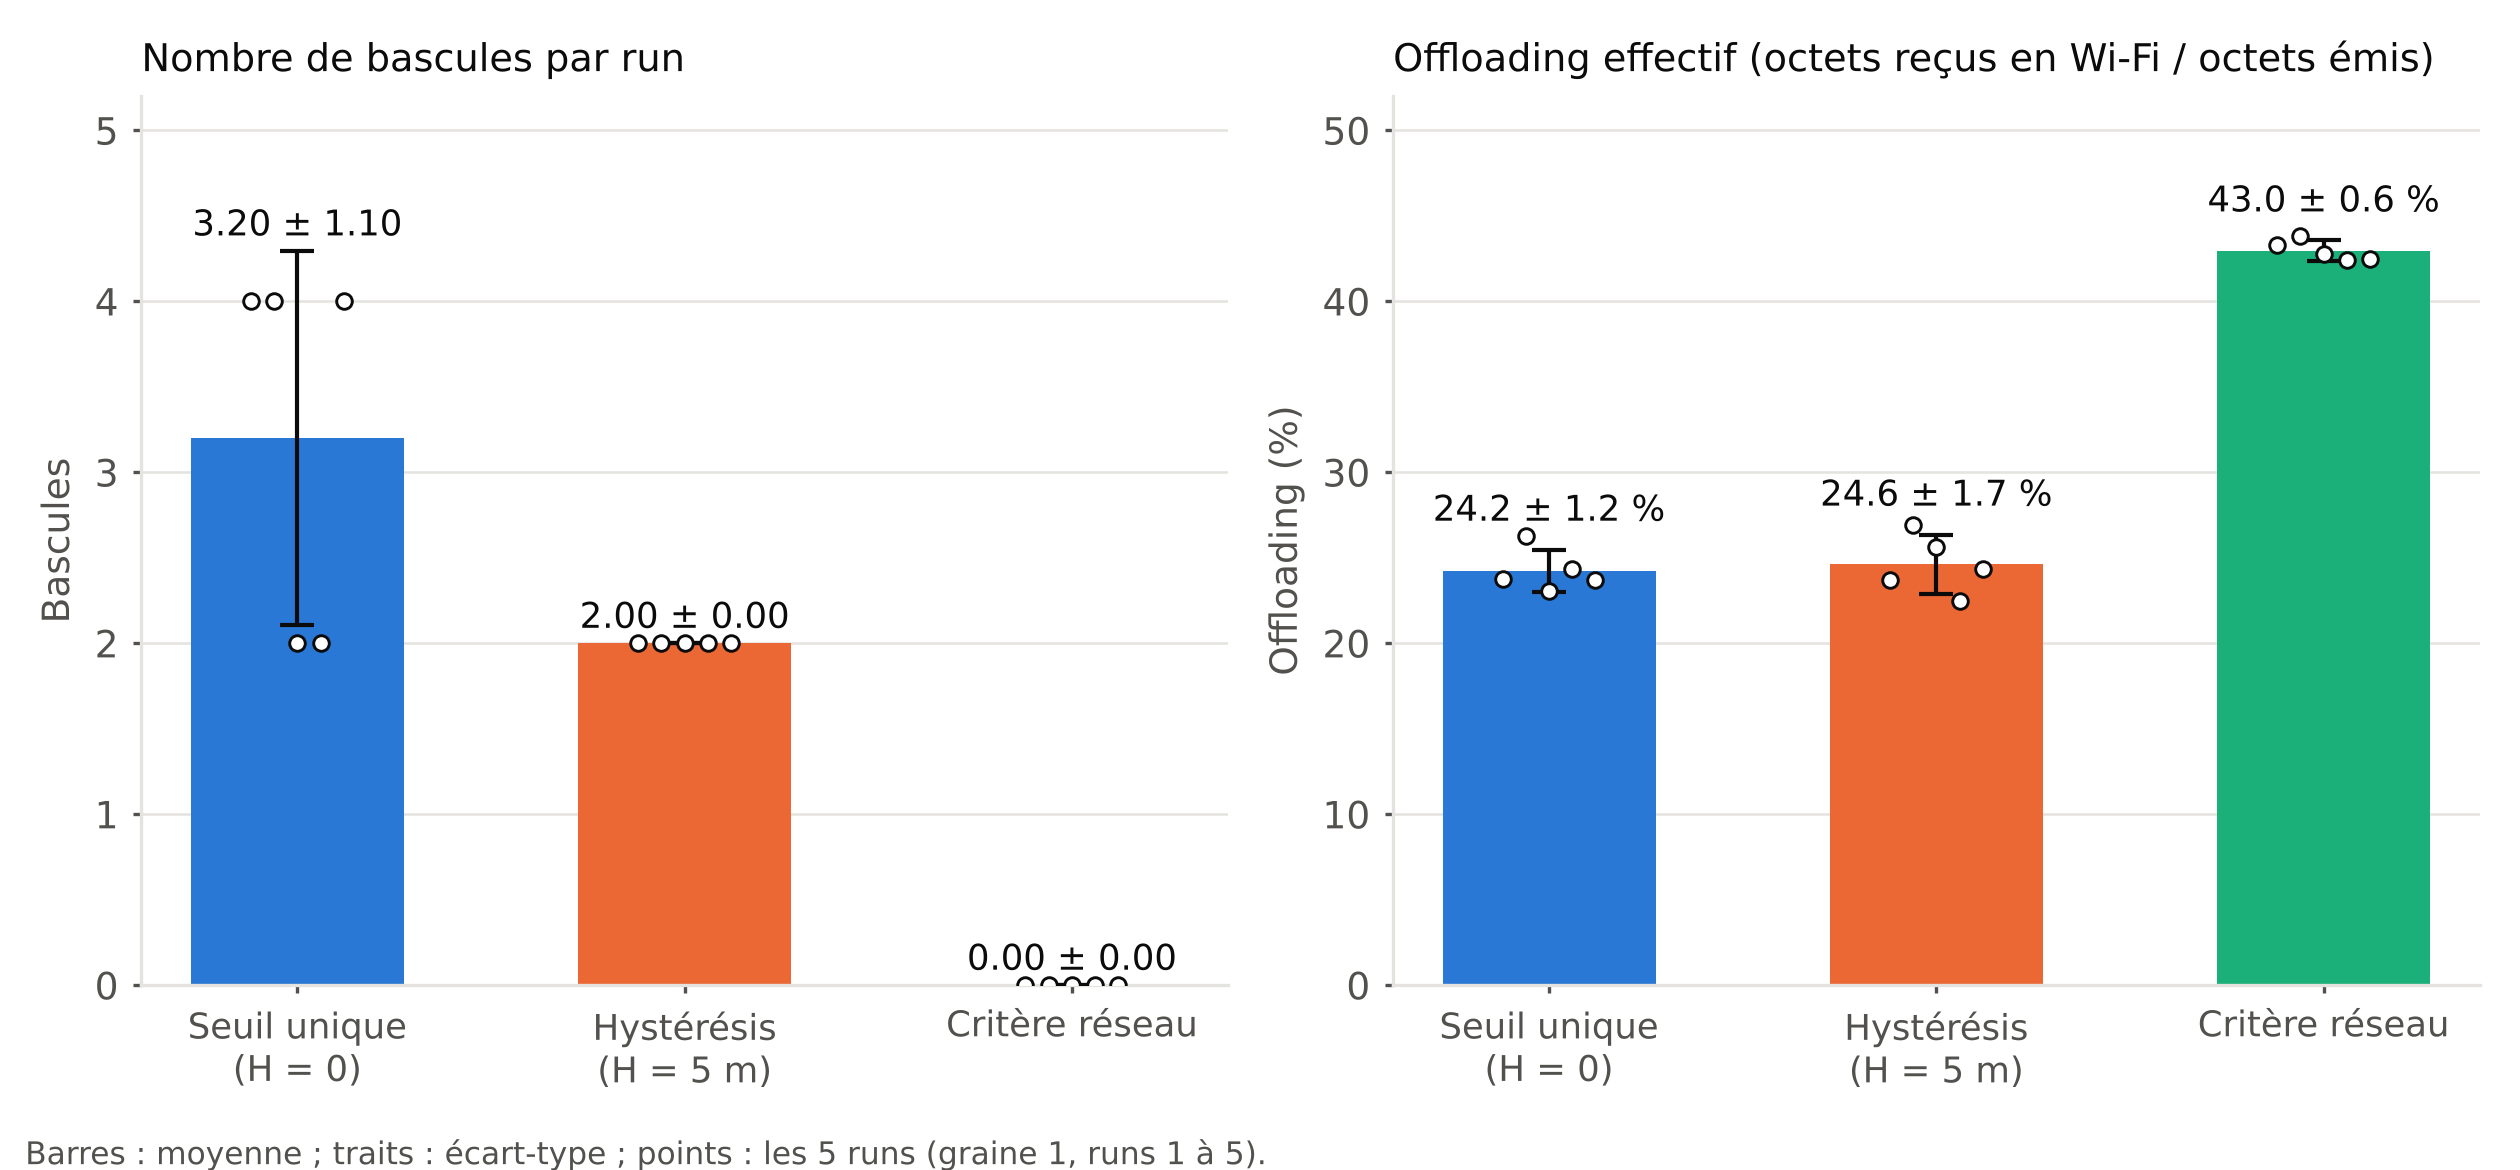
\includegraphics[width=0.7\textwidth]{img/C/pic5_median.png}
      \caption{Nombre de bascules et taux d'offloading par critère (barres + écart-type)}
\end{figure}

\subsection{Analyse}

\paragraph{Nombre de bascules.}
Sans hystérésis, le bruit de mesure de position ($\sigma_d=3$~m) provoque des
bascules supplémentaires lorsque l'UE franchit la frontière du hotspot :
$3{,}20 \pm 1{,}10$ bascules en moyenne, au lieu des deux bascules
attendues (entrée puis sortie). Avec une hystérésis de 5~m, on obtient
exactement deux bascules et aucun ping-pong sur les cinq runs. Ce résultat est
cohérent avec la question B5. Le critère réseau, lui, ne produit aucune
bascule, par construction.

\paragraph{Interruption de service.}
Pour les deux critères terminal, aucune fenêtre de 100~ms n'est passée sous
50\,\% du débit nominal autour des bascules : l'interruption mesurée est nulle.
Seul un pic de délai d'environ 20~ms (contre 13,5~ms en moyenne) est visible.
Ce résultat doit être relativisé : dans NS-3, la bascule se réduit à une
modification de route IP, sans réassociation Wi-Fi ni renégociation d'adresse,
et la résolution de mesure est de 100~ms. Pour le critère réseau, la notion
d'interruption par bascule n'a pas de sens puisqu'il ne bascule jamais en
cours de flux.

\paragraph{Pertes et continuité du service.}
C'est la différence principale entre les approches. Le flux UDP du critère
réseau est « épinglé » sur le Wi-Fi dès t = 1~s. Lorsque l'UE est hors de la
couverture de l'AP, les paquets sont perdus sans qu'aucun mécanisme ne
rebascule le flux vers LTE : on mesure $57{,}04 \pm 0{,}59$\,\% de perte et
44,5~s passées sous le seuil sur 78~s. Les critères terminal, eux, disposent de
LTE comme chemin de repli et n'ont aucune perte. Cette perte provient donc de
l'absence de prise en compte de la mobilité, et non d'un défaut du lien Wi-Fi :
dans l'exécution de contrôle de la question B8, où l'UE reste dans la zone du
hotspot, la perte est nulle.

\paragraph{Taux d'offloading.}
Les critères terminal déchargent environ 24--25\,\% du volume vers le Wi-Fi,
ce qui correspond à la traversée d'une zone de rayon 50~m à 5~m/s. Le critère
réseau atteint environ 43\,\% de volume livré en Wi-Fi : le Wi-Fi reste
utilisable bien au-delà du rayon nominal de 50~m (le déficit de 44,5~s hors
couverture correspond à un rayon effectif de l'ordre de 80~m
Calculé sur les 5 runs par \texttt{rxBytesWifi / (txBytesWifi + txBytesLte)}, il vaut $0{,}43 \pm 0{,}01$.
Le seuil de distance de 50~m est donc conservateur et laisse de la capacité
Wi-Fi inutilisée. En revanche, ce taux plus élevé n'est pas un gain « net » :
il est obtenu au prix de 57\,\% de paquets perdus.

\paragraph{Variabilité entre graines.}
Les écarts-types sont faibles, car la seule source d'aléa est le décalage
latéral $b$ et, pour les critères terminal, le bruit de mesure ; le temps
passé dans le hotspot varie peu avec $b$. Seul le nombre de bascules de
\texttt{dist\_h0} présente une dispersion marquée, ce qui souligne la
sensibilité du seuil unique au bruit de mesure.

\paragraph{Limites de la comparaison.}
\begin{itemize}
  \item Le critère réseau n'a pas de chemin de repli pour le flux UDP, alors
        que les critères terminal en ont un : la comparaison des pertes
        oppose donc deux politiques et pas seulement deux critères.
  \item En mode réseau, un flux TCP supplémentaire circule sur LTE, ce qui n'est
        pas le cas dans les configurations terminal. Le taux d'offloading ne
        porte que sur le flux UDP.
  \item Le shadowing a été désactivé (\texttt{shadowSigma}=0). Lors de nos essais
        avec shadowing activé, aucun paquet n'était livré sur le Wi-Fi ; la
        cause n'a pas été identifiée et la campagne a donc été menée sans
        shadowing.
  \item Cinq graines seulement, sans test statistique inférentiel.
\end{itemize}

\subsection{Quelle approche privilégier ?}

\begin{table}[H]
\centering
\caption{Synthèse comparative des deux familles de critères}
\small
\begin{tabular}{p{3.2cm}p{5.6cm}p{5.6cm}}
\toprule
 & Orienté terminal (distance/RSSI) & Orienté réseau (protocole/débit) \\
\midrule
Mobilité de l'UE & Adapté : suit la couverture réelle et garde LTE en repli & Inadapté pour un UE mobile : aucun suivi de la couverture \\
Nature du trafic & Indifférente à la nature du flux & Exploite le type de flux (UDP débit élevé vs TCP) \\
Stabilité & Risque de ping-pong, atténué par l'hystérésis & Aucune bascule, aucune oscillation \\
Calcul requis & Mesures et décision dans le terminal & Décision centralisée, une fois par flux \\
Information nécessaire & Position ou RSSI de l'UE & Protocole et débit des flux \\
\bottomrule
\end{tabular}
\end{table}

Le critère \textbf{orienté terminal} est préférable lorsque l'UE est mobile ou
lorsque la couverture Wi-Fi est limitée : la décision s'appuie sur l'état
réel du lien et la continuité de service est assurée par LTE. Son coût est un
traitement dans le terminal (mesure et hystérésis) et un risque de bascules
répétées.

Le critère \textbf{orienté réseau} est adapté à des terminaux quasi
statiques ou situés durablement dans la zone Wi-Fi, avec un trafic bien
identifié (par exemple un flux UDP à débit élevé), et lorsque l'opérateur
souhaite centraliser la politique sans solliciter le terminal. Il est
inadapté à un UE mobile tant qu'il n'est pas complété par une réévaluation
périodique du chemin (par exemple à partir du débit mesuré par FlowMonitor),
comme le suggère l'énoncé.

% ---------------------------------------------------------------------
\section{Question 10 : Conclusion sur le Wi-Fi offloading}
% ---------------------------------------------------------------------

Les expériences de la partie B permettent de dégager les conclusions suivantes.

\paragraph{Intérêt pour l'opérateur.}
Lorsque l'UE est dans la zone du hotspot, le Wi-Fi absorbe l'intégralité du
flux UDP de 2~Mb/s, qui n'occupe alors plus les ressources radio LTE. Dans
notre scénario, 24 à 25\,\% du volume est déchargé avec un critère terminal
et jusqu'à environ 43\,\% avec le critère réseau. Il faut toutefois noter
qu'avec un seul UE, nous mesurons une \emph{part du volume} déplacée vers le
Wi-Fi et non une réduction effective de congestion : le gain de charge pour le
réseau LTE n'a pas été quantifié sous charge.

\paragraph{Coût en stabilité.}
Un critère à seuil unique est sensible au bruit de mesure et produit des
bascules supplémentaires ($3{,}2 \pm 1{,}1$ bascules au lieu de 2). L'hystérésis
supprime ce ping-pong, au prix d'une zone de décision plus large qui, si elle
est trop grande, peut empêcher l'accès au Wi-Fi (question B5). Dans la
simulation, les bascules n'entraînent ni perte ni interruption mesurable à la
résolution de 100~ms ; ce résultat ne tient toutefois pas compte de la
réassociation Wi-Fi, de la renégociation IP ou de la rupture éventuelle de
sessions TCP, qui existent dans un réseau réel.

\paragraph{Pertinence du critère de bascule.}
\begin{itemize}
  \item \emph{Distance :} simple à mettre en \oe uvre, mais elle ignore la
        qualité réelle du lien et le seuil nominal sous-exploite la couverture
        effective.
  \item \emph{RSSI :} plus représentatif des conditions radio réelles, avec un
        comportement proche de la distance dans notre canal sans obstacles
        (question B7), mais dont l'intérêt devrait apparaître en milieu urbain
        dense ou en intérieur.
  \item \emph{Protocole/débit décidés côté réseau :} cohérent avec la nature du
        trafic et sans oscillation, mais aveugle à la position de l'UE : il
        provoque 57\,\% de pertes pour un UE mobile qui quitte la couverture.
\end{itemize}

\paragraph{Recommandation.}
Aucun critère isolé n'est satisfaisant pour un terminal mobile. Une approche
combinée est préférable : une politique réseau décide quels flux sont
\emph{éligibles} au Wi-Fi (par protocole et débit), tandis qu'un critère
terminal avec hystérésis, éventuellement fondé sur le RSSI, décide à quel
\emph{moment} utiliser le Wi-Fi, avec LTE comme chemin de repli.

\paragraph{Limites de l'étude.}
Un seul UE et un seul point d'accès, un canal sans shadowing, des bascules
réduites à un changement de route IP, un nombre limité de graines et
l'absence de test statistique inférentiel. Les résultats décrivent le
comportement du scénario simulé et ne se généralisent pas sans campagnes
complémentaires.


\end{document}